\UseRawInputEncoding
%DIF LATEXDIFF DIFFERENCE FILE
%DIF DEL ./old/compiled_v013.tex   Sat Jan 13 18:51:43 2024
%DIF ADD ./compiled.tex            Sat Jan 13 20:06:14 2024

%%%%%%%%%%%%%%%%%%%%%%%%%%%%%%%%%%%%%%%%%%%%%%%%%%%%%%%%%%%%%%%%%%%%%%%%%%%%%%%%
%% SETTINGS
%%%%%%%%%%%%%%%%%%%%%%%%%%%%%%%%%%%%%%%%%%%%%%%%%%%%%%%%%%%%%%%%%%%%%%%%%%%%%%%%
%% Columns
\documentclass[final,3p,times,twocolumn]{elsarticle}
%% Use the options 1p,twocolumn; 3p; 3p,twocolumn; 5p; or 5p,twocolumn
%% for a journal layout:
%% \documentclass[final,1p,times]{elsarticle}
%% \documentclass[final,1p,times,twocolumn]{elsarticle}
%% \documentclass[final,3p,times]{elsarticle}
%% \documentclass[final,3p,times,twocolumn]{elsarticle}
%% \documentclass[final,5p,times]{elsarticle}
%% \documentclass[final,5p,times,twocolumn]{elsarticle}
%% \documentclass[preprint,review,12pt]{elsarticle}

%% Image width
\newlength{\imagewidth}
\newlength{\imagescale}
%% preamble
\usepackage[english]{babel}
\usepackage[table]{xcolor} % For coloring tables
\usepackage{booktabs} % For professional quality tables
\usepackage{colortbl} % For coloring cells in tables
\usepackage{amsmath, amssymb} % For mathematical symbols and environments
\usepackage{amsthm} % For theorem-like environments
\usepackage{lipsum} % just for sample text
\usepackage{natbib}
\usepackage{graphicx}
\usepackage{indentfirst}
\usepackage{bashful}
\usepackage[margin=10pt,font=small,labelfont=bf,labelsep=endash]{caption}
\usepackage{graphicx}
\usepackage{calc}
\usepackage[T1]{fontenc} % [REVISED]
\usepackage[utf8]{inputenc} % [REVISED]
\usepackage{hyperref}
\usepackage{accsupp}
%% Line numbers
\linespread{1.1}
% \linenumbers
% Tables
\usepackage[pass]{geometry}
\usepackage{pdflscape}
\usepackage{csvsimple}
\usepackage{xltabular}
\usepackage{booktabs}
\usepackage{siunitx}
\usepackage{makecell}
\sisetup{round-mode=figures,round-precision=3}
\renewcommand\theadfont{\bfseries}
\renewcommand\theadalign{c}
\newcolumntype{C}[1]{>{\centering\arraybackslash}m{#1}}
\renewcommand{\arraystretch}{1.5}
\definecolor{lightgray}{gray}{0.95}

%% Diff
\usepackage{xcolor}
% Define commands for highlighting
% diff
\usepackage[most]{tcolorbox} % for boxes with transparency
% Define colors with transparency (opacity value)
\definecolor{GreenBG}{rgb}{0,1,0}
\definecolor{RedBG}{rgb}{1,0,0}
% Define tcolorbox environments for highlighting
\newtcbox{\greenhighlight}[1][]{%
  on line,
  colframe=GreenBG,
  colback=GreenBG!50!white, % 50% transparent green
  boxrule=0pt,
  arc=0pt,
  boxsep=0pt,
  left=1pt,
  right=1pt,
  top=2pt,
  bottom=2pt,
  tcbox raise base
}
\newtcbox{\redhighlight}[1][]{%
  on line,
  colframe=RedBG,
  colback=RedBG!50!white, % 50% transparent red
  boxrule=0pt,
  arc=0pt,
  boxsep=0pt,
  left=1pt,
  right=1pt,
  top=2pt,
  bottom=2pt,
  tcbox raise base
}
\newcommand{\REDSTARTS}{\color{red}}
\newcommand{\REDENDS}{\color{black}}
\newcommand{\GREENSTARTS}{\color{green}}
\newcommand{\GREENENDS}{\color{black}}
%%%%%%%%%%%%%%%%%%%%%%%%%%%%%%%%%%%%%%%%%%%%%%%%%%%%%%%%%%%%%%%%%%%%%%%%%%%%%%%%
%% JOURNAL NAME
%%%%%%%%%%%%%%%%%%%%%%%%%%%%%%%%%%%%%%%%%%%%%%%%%%%%%%%%%%%%%%%%%%%%%%%%%%%%%%%%
\journal{Heliyon}
%%%%%%%%%%%%%%%%%%%%%%%%%%%%%%%%%%%%%%%%%%%%%%%%%%%%%%%%%%%%%%%%%%%%%%%%%%%%%%%%
%% DOCUMENT STARTS
%%%%%%%%%%%%%%%%%%%%%%%%%%%%%%%%%%%%%%%%%%%%%%%%%%%%%%%%%%%%%%%%%%%%%%%%%%%%%%%%
%DIF PREAMBLE EXTENSION ADDED BY LATEXDIFF
%DIF UNDERLINE PREAMBLE %DIF PREAMBLE
\RequirePackage[normalem]{ulem} %DIF PREAMBLE
\RequirePackage{color}\definecolor{RED}{rgb}{1,0,0}\definecolor{BLUE}{rgb}{0,0,1} %DIF PREAMBLE
\providecommand{\DIFaddtex}[1]{{\protect\color{blue}\uwave{#1}}} %DIF PREAMBLE
\providecommand{\DIFdeltex}[1]{{\protect\color{red}\sout{#1}}}                      %DIF PREAMBLE
%DIF SAFE PREAMBLE %DIF PREAMBLE
\providecommand{\DIFaddbegin}{} %DIF PREAMBLE
\providecommand{\DIFaddend}{} %DIF PREAMBLE
\providecommand{\DIFdelbegin}{} %DIF PREAMBLE
\providecommand{\DIFdelend}{} %DIF PREAMBLE
\providecommand{\DIFmodbegin}{} %DIF PREAMBLE
\providecommand{\DIFmodend}{} %DIF PREAMBLE
%DIF FLOATSAFE PREAMBLE %DIF PREAMBLE
\providecommand{\DIFaddFL}[1]{\DIFadd{#1}} %DIF PREAMBLE
\providecommand{\DIFdelFL}[1]{\DIFdel{#1}} %DIF PREAMBLE
\providecommand{\DIFaddbeginFL}{} %DIF PREAMBLE
\providecommand{\DIFaddendFL}{} %DIF PREAMBLE
\providecommand{\DIFdelbeginFL}{} %DIF PREAMBLE
\providecommand{\DIFdelendFL}{} %DIF PREAMBLE
%DIF HYPERREF PREAMBLE %DIF PREAMBLE
\providecommand{\DIFadd}[1]{\texorpdfstring{\DIFaddtex{#1}}{#1}} %DIF PREAMBLE
\providecommand{\DIFdel}[1]{\texorpdfstring{\DIFdeltex{#1}}{}} %DIF PREAMBLE
\newcommand{\DIFscaledelfig}{0.5}
%DIF HIGHLIGHTGRAPHICS PREAMBLE %DIF PREAMBLE
\RequirePackage{settobox} %DIF PREAMBLE
\RequirePackage{letltxmacro} %DIF PREAMBLE
\newsavebox{\DIFdelgraphicsbox} %DIF PREAMBLE
\newlength{\DIFdelgraphicswidth} %DIF PREAMBLE
\newlength{\DIFdelgraphicsheight} %DIF PREAMBLE
% store original definition of \includegraphics %DIF PREAMBLE
\LetLtxMacro{\DIFOincludegraphics}{\includegraphics} %DIF PREAMBLE
\newcommand{\DIFaddincludegraphics}[2][]{{\color{blue}\fbox{\DIFOincludegraphics[#1]{#2}}}} %DIF PREAMBLE
\newcommand{\DIFdelincludegraphics}[2][]{% %DIF PREAMBLE
\sbox{\DIFdelgraphicsbox}{\DIFOincludegraphics[#1]{#2}}% %DIF PREAMBLE
\settoboxwidth{\DIFdelgraphicswidth}{\DIFdelgraphicsbox} %DIF PREAMBLE
\settoboxtotalheight{\DIFdelgraphicsheight}{\DIFdelgraphicsbox} %DIF PREAMBLE
\scalebox{\DIFscaledelfig}{% %DIF PREAMBLE
\parbox[b]{\DIFdelgraphicswidth}{\usebox{\DIFdelgraphicsbox}\\[-\baselineskip] \rule{\DIFdelgraphicswidth}{0em}}\llap{\resizebox{\DIFdelgraphicswidth}{\DIFdelgraphicsheight}{% %DIF PREAMBLE
\setlength{\unitlength}{\DIFdelgraphicswidth}% %DIF PREAMBLE
\begin{picture}(1,1)% %DIF PREAMBLE
\thicklines\linethickness{2pt} %DIF PREAMBLE
{\color[rgb]{1,0,0}\put(0,0){\framebox(1,1){}}}% %DIF PREAMBLE
{\color[rgb]{1,0,0}\put(0,0){\line( 1,1){1}}}% %DIF PREAMBLE
{\color[rgb]{1,0,0}\put(0,1){\line(1,-1){1}}}% %DIF PREAMBLE
\end{picture}% %DIF PREAMBLE
}\hspace*{3pt}}} %DIF PREAMBLE
} %DIF PREAMBLE
\LetLtxMacro{\DIFOaddbegin}{\DIFaddbegin} %DIF PREAMBLE
\LetLtxMacro{\DIFOaddend}{\DIFaddend} %DIF PREAMBLE
\LetLtxMacro{\DIFOdelbegin}{\DIFdelbegin} %DIF PREAMBLE
\LetLtxMacro{\DIFOdelend}{\DIFdelend} %DIF PREAMBLE
\DeclareRobustCommand{\DIFaddbegin}{\DIFOaddbegin \let\includegraphics\DIFaddincludegraphics} %DIF PREAMBLE
\DeclareRobustCommand{\DIFaddend}{\DIFOaddend \let\includegraphics\DIFOincludegraphics} %DIF PREAMBLE
\DeclareRobustCommand{\DIFdelbegin}{\DIFOdelbegin \let\includegraphics\DIFdelincludegraphics} %DIF PREAMBLE
\DeclareRobustCommand{\DIFdelend}{\DIFOaddend \let\includegraphics\DIFOincludegraphics} %DIF PREAMBLE
\LetLtxMacro{\DIFOaddbeginFL}{\DIFaddbeginFL} %DIF PREAMBLE
\LetLtxMacro{\DIFOaddendFL}{\DIFaddendFL} %DIF PREAMBLE
\LetLtxMacro{\DIFOdelbeginFL}{\DIFdelbeginFL} %DIF PREAMBLE
\LetLtxMacro{\DIFOdelendFL}{\DIFdelendFL} %DIF PREAMBLE
\DeclareRobustCommand{\DIFaddbeginFL}{\DIFOaddbeginFL \let\includegraphics\DIFaddincludegraphics} %DIF PREAMBLE
\DeclareRobustCommand{\DIFaddendFL}{\DIFOaddendFL \let\includegraphics\DIFOincludegraphics} %DIF PREAMBLE
\DeclareRobustCommand{\DIFdelbeginFL}{\DIFOdelbeginFL \let\includegraphics\DIFdelincludegraphics} %DIF PREAMBLE
\DeclareRobustCommand{\DIFdelendFL}{\DIFOaddendFL \let\includegraphics\DIFOincludegraphics} %DIF PREAMBLE
%DIF LISTINGS PREAMBLE %DIF PREAMBLE
\RequirePackage{listings} %DIF PREAMBLE
\RequirePackage{color} %DIF PREAMBLE
\lstdefinelanguage{DIFcode}{ %DIF PREAMBLE
%DIF DIFCODE_UNDERLINE %DIF PREAMBLE
  moredelim=[il][\color{red}\sout]{\%DIF\ <\ }, %DIF PREAMBLE
  moredelim=[il][\color{blue}\uwave]{\%DIF\ >\ } %DIF PREAMBLE
} %DIF PREAMBLE
\lstdefinestyle{DIFverbatimstyle}{ %DIF PREAMBLE
	language=DIFcode, %DIF PREAMBLE
	basicstyle=\ttfamily, %DIF PREAMBLE
	columns=fullflexible, %DIF PREAMBLE
	keepspaces=true %DIF PREAMBLE
} %DIF PREAMBLE
\lstnewenvironment{DIFverbatim}{\lstset{style=DIFverbatimstyle}}{} %DIF PREAMBLE
\lstnewenvironment{DIFverbatim*}{\lstset{style=DIFverbatimstyle,showspaces=true}}{} %DIF PREAMBLE
%DIF END PREAMBLE EXTENSION ADDED BY LATEXDIFF

\begin{document}

%%%%%%%%%%%%%%%%%%%%%%%%%%%%%%%%%%%%%%%%%%%%%%%%%%%%%%%%%%%%%%%%%%%%%%%%%%%%%%%%
%% Frontmatter
%%%%%%%%%%%%%%%%%%%%%%%%%%%%%%%%%%%%%%%%%%%%%%%%%%%%%%%%%%%%%%%%%%%%%%%%%%%%%%%%
\begin{frontmatter}
\begin{highlights}
\pdfbookmark[1]{Highlights}{highlights}

\item Neural trajectories in the hippocampus exhibited greater variability during a working memory (WM) task compared to those in the entorhinal cortex and amygdala regions.

\item The distance of neural trajectories between encoding and retrieval states in the hippocampus was memory-load dependent during a WM task.


\item Hippocampal neural trajectories fluctuated between the encoding and retrieval states in a task-dependent manner during both baseline and sharp-wave ripple (SWR) periods.

\item Hippocampal neural trajectories shifted from encoding to retrieval states during SWR period.

\end{highlights}\title{
Hippocampal neural fluctuations between memory encoding and retrieval states during a working memory task in humans
}\author[1]{Yusuke Watanabe\corref{cor1}}
\author[2,3,4]{Yuji Ikegaya}
\author[1,5]{Takufumi Yanagisawa}

\address[1]{Institute for Advanced Cocreation studies, Osaka University, 2-2 Yamadaoka, Suita, 565-0871, Osaka, Japan}
\address[2]{Graduate School of Pharmaceutical Sciences, The University of Tokyo, 7-3-1 Hongo, Tokyo, 113-0033, Japan}
\address[3]{Institute for AI and Beyond, The University of Tokyo, 7-3-1 Hongo, Tokyo, 113-0033, Japan}
\address[4]{Center for Information and Neural Networks, National Institute of Information and Communications Technology, 1-4 Yamadaoka, Suita City, 565-0871, Osaka, Japan}
\address[5]{Department of Neurosurgery, Osaka University Graduate School of Medicine, 2-2 Yamadaoka, Osaka, 565-0871, Japan}

\cortext[cor1]{Corresponding author. Tel: +81-6-6879-3652}%%Graphical abstract
%\pdfbookmark[1]{Graphical Abstract}{graphicalabstract}        
%\begin{graphicalabstract}
%\includegraphics{grabs}
%\end{graphicalabstract}
\begin{abstract}
\pdfbookmark[1]{Abstract}{abstract}
Working memory (WM) plays a critical role in \DIFdelbegin \DIFdel{many }\DIFdelend \DIFaddbegin \DIFadd{various }\DIFaddend cognitive functions, but the intricate neural mechanisms that support its operation remain elusive. Specifically, while the hippocampus and sharp-wave ripple complexes (SWRs) -- brief, synchronous neural oscillation observed in the hippocampus -- are recognized for their roles in memory consolidation and retrieval, their involvement in WM tasks has not yet been defined. \DIFdelbegin \DIFdel{Current research suggests that during WM tasks}\DIFdelend \DIFaddbegin \DIFadd{Here we show that during a WM task}\DIFaddend , multiunit activity patterns in the hippocampus display distinctive dynamics, particularly during SWR periods. This study analyzed a dataset derived from intracranial electroencephalogram recordings \DIFdelbegin \DIFdel{made }\DIFdelend \DIFaddbegin \DIFadd{conducted }\DIFaddend in the medial temporal lobe (MTL) of nine individuals with epilepsy during an eight-second Sternberg task. We applied Gaussian-process factor analysis to determine low-dimensional neural representations, or 'trajectories,' within the MTL regions while performing the WM task. The results \DIFdelbegin \DIFdel{indicate }\DIFdelend \DIFaddbegin \DIFadd{revealed }\DIFaddend significant variations in the hippocampus' neural trajectories compared to those in the entorhinal cortex and amygdala. Additionally, the distance of the trajectory between the encoding and retrieval phases was dependent on memory load. Importantly, hippocampal trajectories during the retrieval phase demonstrated \DIFdelbegin \DIFdel{variations }\DIFdelend \DIFaddbegin \DIFadd{fluctuations }\DIFaddend between encoding and retrieval stages based on task type, particularly showing \DIFdelbegin \DIFdel{shifts }\DIFdelend \DIFaddbegin \DIFadd{transient shift }\DIFaddend from encoding to retrieval states during SWRs. These findings underline the hippocampus's essential function in performing WM tasks and propose \DIFdelbegin \DIFdel{an intriguing }\DIFdelend \DIFaddbegin \DIFadd{a }\DIFaddend hypothesis for future research: the functional state of the hippocampus transition from encoding to retrieval during SWRs.
\end{abstract}% \pdfbookmark[1]{Keywords}{keywords}                
\begin{keyword}
working memory \sep memory load \sep hippocampus \sep sharp-wave ripples \sep humans
\end{keyword}
\end{frontmatter}

%%%%%%%%%%%%%%%%%%%%%%%%%%%%%%%%%%%%%%%%%%%%%%%%%%%%%%%%%%%%%%%%%%%%%%%%%%%%%%%%
%% IMRaD
%%%%%%%%%%%%%%%%%%%%%%%%%%%%%%%%%%%%%%%%%%%%%%%%%%%%%%%%%%%%%%%%%%%%%%%%%%%%%%%%

%%%%%%%%%%%%%%%%%%%%%%%%%%%%%%%%%%%%%%%%%%%%%%%%%%%%%%%%%%%%%%%%%%%%%%%%%%%%%%%%
%% INTRODUCTION
%%%%%%%%%%%%%%%%%%%%%%%%%%%%%%%%%%%%%%%%%%%%%%%%%%%%%%%%%%%%%%%%%%%%%%%%%%%%%%%%
\section{Introduction}
Working memory (WM) significantly influences everyday life, and the neural bases of this cognitive process continue to be the subject of intensive research. One key focus of this research is the hippocampus, a structure integral to memory functions \cite{scoville_loss_1957} \cite{squire_legacy_2009}  \cite{boran_persistent_2019} \cite{kaminski_persistently_2017} \cite{kornblith_persistent_2017} \cite{faraut_dataset_2018} \cite{borders_hippocampus_2022} \cite{li_functional_2023} \cite{dimakopoulos_information_2022}. A \DIFdelbegin \DIFdel{thorough }\DIFdelend \DIFaddbegin \DIFadd{deeper }\DIFaddend understanding of the hippocampus's role in working memory is \DIFdelbegin \DIFdel{essential }\DIFdelend \DIFaddbegin \DIFadd{not only crucial }\DIFaddend for advancing our knowledge \DIFdelbegin \DIFdel{of cognitive processes }%DIFDELCMD < [%%%
\DIFdel{CHECKME>}%DIFDELCMD < ]%%%
\DIFdel{and fostering advancements in cognitive training and interventions}%DIFDELCMD < [%%%
\DIFdel{<CHECKME ENDS}%DIFDELCMD < ]%%%
\DIFdelend \DIFaddbegin \DIFadd{but also potentially for enhancing cognitive abilities}\DIFaddend .
\\
\indent
Current evidence suggests that a transient, synchronized oscillation, called sharp-wave ripple (SWR) \cite{buzsaki_hippocampal_2015}, is associated with several cognitive functions. These include memory replay \cite{wilson_reactivation_1994} \cite{nadasdy_replay_1999} \cite{lee_memory_2002} \cite{diba_forward_2007} \cite{davidson_hippocampal_2009}, memory consolidation \cite{girardeau_selective_2009} \cite{ego-stengel_disruption_2010} \cite{fernandez-ruiz_long-duration_2019} \cite{kim_corticalhippocampal_2022}, memory recall \cite{wu_hippocampal_2017} \cite{norman_hippocampal_2019} \cite{norman_hippocampal_2021}, and neural plasticity \cite{behrens_induction_2005} \cite{norimoto_hippocampal_2018}. \DIFdelbegin \DIFdel{This association suggests }\DIFdelend \DIFaddbegin \DIFadd{These associations suggest }\DIFaddend that SWR may be a \DIFdelbegin \DIFdel{crucial part }\DIFdelend \DIFaddbegin \DIFadd{fundamental computational manifestation }\DIFaddend of hippocampal processing\DIFdelbegin \DIFdel{that contributes }\DIFdelend \DIFaddbegin \DIFadd{, contributing }\DIFaddend to working memory performance \DIFaddbegin \DIFadd{as well}\DIFaddend . However, research on the effects of SWRs on working memory is relatively scarce \cite{jadhav_awake_2012}, and is predominantly limited to rodent models engaged in navigation tasks, where the timing of memory acquisition and recall is not clearly defined.
\\
\indent
Recent studies have found low-dimensional representations in the hippocampal neurons \DIFdelbegin \DIFdel{during WM tasks}\DIFdelend \DIFaddbegin \DIFadd{can explain WM task performances}\DIFaddend . Specifically, the firing patterns of place cells \cite{okeefe_hippocampus_1971} \cite{okeefe_place_1976} \cite{ekstrom_cellular_2003} \cite{kjelstrup_finite_2008} \cite{harvey_intracellular_2009}, found in the hippocampus, have been identified within a dynamic, nonlinear three-dimensional hyperbolic space in rats \cite{zhang_hippocampal_2022}. Additionally, grid cells in the entorhinal cortex (EC), which is the main pathway to the hippocampus \cite{naber_reciprocal_2001} \cite{van_strien_anatomy_2009} \cite{strange_functional_2014}, exhibited a toroidal geometry during exploration in rats \cite{gardner_toroidal_2022}. However, these studies are limited by their focus on spatial navigation tasks in rodents, affecting the temporal resolution of WM tasks\DIFdelbegin %DIFDELCMD < [%%%
\DIFdel{CHECKME>}%DIFDELCMD < ]%%%
\DIFdel{such as }\DIFdelend \DIFaddbegin \DIFadd{. To illustrate, }\DIFaddend the timing of \DIFdelbegin \DIFdel{information acquisition and recall}%DIFDELCMD < [%%%
\DIFdel{<CHECKME ENDS}%DIFDELCMD < ]%%%
\DIFdel{. The }\DIFdelend \DIFaddbegin \DIFadd{when an animal acquires information is ambiguous in these settings. Therefore, the }\DIFaddend applicability of these findings to human subjects and \DIFdelbegin \DIFdel{beyond navigation tasks still needs to be confirmed}\DIFdelend \DIFaddbegin \DIFadd{tasks beyond navigation still requires confirmation}\DIFaddend .
\\
\indent
Considering these \DIFdelbegin \DIFdel{aspects, the present study aims to investigate }\DIFdelend \DIFaddbegin \DIFadd{factors, this study investigates }\DIFaddend the hypothesis that hippocampal neurons \DIFdelbegin \DIFdel{display distinctive patterns of activity or }\DIFdelend \DIFaddbegin \DIFadd{show unique }\DIFaddend 'neural trajectories' in low-dimensional spaces, particularly during SWR periods, in response to WM tasks. To test this hypothesis, we \DIFdelbegin \DIFdel{used }\DIFdelend \DIFaddbegin \DIFadd{employed }\DIFaddend a dataset of patients performing an eight-second Sternberg task (1 s for fixation, 2 s for encoding, 3 s for maintenance, and 2 s for retrieval) with high temporal resolution. Intracranial electroencephalography (iEEG) signals within the medial temporal lobe (MTL) were recorded for these patients \cite{boran_dataset_2020}. To examine low-dimensional neural trajectories, we utilized Gaussian-process factor analysis (GPFA), an established method for analyzing neural population dynamics \cite{yu_gaussian-process_2009}.
\label{sec:introduction}
%%%%%%%%%%%%%%%%%%%%%%%%%%%%%%%%%%%%%%%%%%%%%%%%%%%%%%%%%%%%%%%%%%%%%%%%%%%%%%%%
%% METHODS
%%%%%%%%%%%%%%%%%%%%%%%%%%%%%%%%%%%%%%%%%%%%%%%%%%%%%%%%%%%%%%%%%%%%%%%%%%%%%%%%
\section{Methods}
\subsection{Dataset}
The dataset \DIFdelbegin \DIFdel{employed }\DIFdelend \DIFaddbegin \DIFadd{used }\DIFaddend in this study\DIFdelbegin \DIFdel{was publicly availableand consisted of }\DIFdelend \DIFaddbegin \DIFadd{, which is publicly available, comprises }\DIFaddend nine epilepsy patients performing a modified Sternberg task \cite{boran_dataset_2020}. This task \DIFdelbegin \DIFdel{encompassed }\DIFdelend \DIFaddbegin \DIFadd{includes }\DIFaddend four phases: fixation (1s), encoding (2s), maintenance (3s), and retrieval (2s). During the encoding phase, participants were presented with \DIFaddbegin \DIFadd{a set of }\DIFaddend four, six, or eight alphabet letters\DIFdelbegin \DIFdel{, defined as the set size. They }%DIFDELCMD < [%%%
\DIFdel{FIXME>}%DIFDELCMD < ]%%%
\DIFdel{were required to}%DIFDELCMD < [%%%
\DIFdel{<FIXME}%DIFDELCMD < ] %%%
\DIFdel{ascertain }\DIFdelend \DIFaddbegin \DIFadd{. They were then tasked with determining }\DIFaddend whether a probe letter \DIFdelbegin \DIFdel{shown }\DIFdelend \DIFaddbegin \DIFadd{displayed }\DIFaddend during the retrieval phase had \DIFdelbegin \DIFdel{appeared before }\DIFdelend \DIFaddbegin \DIFadd{previously appeared }\DIFaddend (the correct \DIFdelbegin \DIFdel{choice for the }\DIFdelend \DIFaddbegin \DIFadd{response for }\DIFaddend Match IN task) or not (the correct \DIFdelbegin \DIFdel{choice for the }\DIFdelend \DIFaddbegin \DIFadd{response for }\DIFaddend Mismatch OUT task). Intracranial electroencephalography (iEEG) signals were captured with a 32 kHz sampling rate within a 0.5--5,000 Hz frequency range, using depth electrodes in medial temporal lobe (MTL) regions: the anterior head of the left and right hippocampus (AHL and AHR), the posterior body of the hippocampus (PHL and PHR), the entorhinal cortex (ECL and ECR), and the amygdala (AL and AR), as depicted in Figure~\ref{fig:01}A and Table~\ref{tab:01}. The iEEG signals were subsequently downsampled to 2 kHz. Correlations between variables such as set size and correct rate were examined (Figure~\ref{fig:s01}S1). Multiunit spike timings were determined via a spike sorting algorithm \cite{niediek_reliable_2016} using the Combinato package (\url{https://github.com/jniediek/combinato})(Figure~\ref{fig:01}C).

\subsection{Calculation of neural trajectories using GPFA}
Neural trajectories, also referred to as 'factors'\DIFdelbegin \DIFdel{(Figure~\ref{fig:01}D)}\DIFdelend , in the hippocampus, EC, and amygdala were determined using GPFA \cite{yu_gaussian-process_2009} applied to the multiunit activity data for each session, performed with the elephant package (\url{https://elephant.readthedocs.io/en/latest/reference/gpfa.html}). The bin size was set to 50 ms, without overlaps. Each factor was z-normalized across all sessions, and the Euclidean distance from the origin ($O$) was then computed\DIFdelbegin \DIFdel{(Figure~\ref{fig:01}E).
}%DIFDELCMD < 

%DIFDELCMD < %%%
\DIFdelend \DIFaddbegin \DIFadd{.
}\\
\indent
\DIFaddend For each trajectory within a region such as AHL, geometric medians ($\mathrm{g_{F}}$ for fixation, $\mathrm{g_{E}}$ for encoding, $\mathrm{g_{M}}$ for maintenance, and $\mathrm{g_{R}}$ for retrieval phase) were calculated by determining the median coordinates of the trajectory during the four phases\DIFdelbegin \DIFdel{(Figure~\ref{fig:01}D)}\DIFdelend . An optimal GPFA dimensionality was found to be three using the elbow method obtained by examining the log-likelihood values through a three-fold cross-validation approach (Figure~\ref{fig:02}B).

\subsection{Identifying SWR candidates from hippocampal regions}
Potential SWR events within the hippocampus were detected using a widely used method \cite{liu_consensus_2022}. LFP signals from a region of interest (ROI) like AHL, were re-referenced by deducting the averaged signal from locations outside the ROI (for instance, AHR, PHL, PHR, ECL, ECR, AL, and AR)\DIFdelbegin \DIFdel{(see Figure~\ref{fig:01}A)}\DIFdelend . The re-referenced LFP signals were then filtered with a ripple-band filter (80--140 Hz) to determine SWR candidates, marked as $\textrm{SWR}^+$ candidates\DIFdelbegin \DIFdel{(see Figure~\ref{fig:01}B)}\DIFdelend . SWR detection was carried out using a published tool (\url{https://github.com/Eden-Kramer-Lab/ripple_detection}) \cite{kay_hippocampal_2016}, with the bandpass range adjusted to 80--140 Hz for humans \cite{norman_hippocampal_2019} \cite{norman_hippocampal_2021}, unlike the initial 150--250 Hz range typically applied to rodents.
\DIFdelbegin %DIFDELCMD < 

%DIFDELCMD < %%%
\DIFdelend \DIFaddbegin \\
\indent
\DIFaddend Control events for $\textrm{SWR}^+$ candidates, labeled as $\textrm{SWR}^-$ candidates, were detected by randomly shuffling the timestamps of $\textrm{SWR}^+$ candidates across all trials and subjects. The resulting $\textrm{SWR}^+/\textrm{SWR}^-$ candidates were then visually inspected\DIFdelbegin \DIFdel{(Figure~\ref{fig:01})}\DIFdelend .

\subsection{Defining SWRs from putative hippocampal CA1 regions}
\DIFaddbegin \DIFadd{Potential }\DIFaddend SWRs were differentiated from SWR candidates in putative CA1 \DIFaddbegin \DIFadd{(cornu Ammonis 1) }\DIFaddend regions. These regions were initially defined as follows: $\textrm{SWR}^+/\textrm{SWR}^-$ candidates in the hippocampus were projected into a two-dimensional space based on overlapping spike counts per unit using a supervised method, UMAP (Uniform Manifold Approximation and Projection) \cite{mcinnes_umap_2018}\DIFdelbegin \DIFdel{(Figure~\ref{fig:04}A)}\DIFdelend . Clustering validation was performed by calculating the silhouette score \cite{rousseeuw_silhouettes_1987} from clustered samples\DIFdelbegin \DIFdel{(Table~\ref{tab:02})}\DIFdelend . Regions in the hippocampus, which scored above 0.6 on average across sessions (75th percentile)\DIFdelbegin \DIFdel{(Figure~\ref{fig:04}B)}\DIFdelend , were identified as putative CA1 regions, resulting in the identification of five electrode positions from five patients\DIFdelbegin \DIFdel{(Table~\ref{tab:03}).
}%DIFDELCMD < 

%DIFDELCMD < %%%
\DIFdelend \DIFaddbegin \DIFadd{.
}\\
\indent
\DIFaddend $\textrm{SWR}^+/\textrm{SWR}^-$ candidates in these predetermined CA1 regions were categorized as $\textrm{SWR}^+/\textrm{SWR}^-$, and thus they no longer retained their candidate status. The duration and ripple band peak amplitude of SWRs were found to follow log-normal distributions\DIFdelbegin \DIFdel{(Figure~\ref{fig:04}C \& E)}\DIFdelend . Each time period of SWR was partitioned relative to the time from the SWR center into pre- (at $-800$ to $-300$ ms from the SWR center), mid- (at $-250$ to $+250$ ms), and post-SWR (at $+300$ to $+800$ ms) times.
\DIFdelbegin %DIFDELCMD < 

%DIFDELCMD < %%%
\DIFdelend \DIFaddbegin \\
\indent
\DIFaddend \subsection{Statistical evaluation}
Both the Brunner--Munzel test and the Kruskal-Wallis test were executed using the SciPy package in Python \cite{virtanen_scipy_2020}. Correlational analysis was conducted by determining the rank of the observed correlation coefficient within its associated set-size-shuffled surrogate using a customized Python script. The bootstrap test was implemented with an in-house Python script.
\DIFdelbegin %DIFDELCMD < 

%DIFDELCMD < %%%
\DIFdelend \label{sec:methods}
%%%%%%%%%%%%%%%%%%%%%%%%%%%%%%%%%%%%%%%%%%%%%%%%%%%%%%%%%%%%%%%%%%%%%%%%%%%%%%%%
%% RESULTS
%%%%%%%%%%%%%%%%%%%%%%%%%%%%%%%%%%%%%%%%%%%%%%%%%%%%%%%%%%%%%%%%%%%%%%%%%%%%%%%%
\section{Results}
\subsection{iEEG recording and neural trajectory in MTL regions during a Sternberg task}
Our analysis employed a publicly accessible dataset \cite{boran_dataset_2020}, which comprises LFP signals (Figure~\ref{fig:01}A) from MTL regions (Table~\ref{tab:01}) recorded during the execution of a modified Sternberg task. We extracted SWR$^+$ candidates from LFP signals that were filtered in the 80--140 Hz ripple band (Figure~\ref{fig:01}B), originating in all hippocampal regions (refer to Methods section). Meanwhile, SWR$^-$ candidates\DIFaddbegin \DIFadd{, control events for SWR$^+$ candidates, }\DIFaddend were defined at the same timestamps but distributed across different trials (Figure~\ref{fig:01}). The dataset also encompassed multiunit spikes (Figure~\ref{fig:01}C), recognized via a spike sorting algorithm \cite{niediek_reliable_2016}. Employing GPFA \cite{yu_gaussian-process_2009}, we applied this to 50-ms windows of binned multiunit activity without overlaps to determine the neural trajectories, or factors, of MTL regions by session and region (Figure~\ref{fig:01}D). We normalized each factor per session and region, for instance, session \#2 in AHL of subject \#1. We then calculated the Euclidean distance from the origin ($O$) (Figure~\ref{fig:01}E).

\subsection{Hippocampal neural trajectory correlation with a Sternberg task}
Figure~\ref{fig:02}A exhibits a distribution of median neural trajectories, comprising 50 trials, within the three main factor spaces. Utilizing the elbow method, we established the optimal embedding dimension for the GPFA model as three (Figure~\ref{fig:02}B). The trajectory distance from the origin ($O$) \DIFdelbegin \DIFdel{-- }\DIFdelend \DIFaddbegin \DIFadd{--- }\DIFaddend represented as $\mathrm{\lVert g_{F} \rVert}$, $\mathrm{\lVert g_{E} \rVert}$, $\mathrm{\lVert g_{M} \rVert}$, and $\mathrm{\lVert g_{R} \rVert}$ \DIFdelbegin \DIFdel{–  }\DIFdelend \DIFaddbegin \DIFadd{--- }\DIFaddend in the hippocampus surpassed the corresponding distances in the EC and amygdala (Figure~\ref{fig:02}C \& D).\footnote{Hippocampus: Distance = 1.11 [1.01], median [IQR], \textit{n} = 195,681 timepoints; EC: Distance = 0.94 [1.10], median [IQR], \textit{n} = 133,761 timepoints; Amygdala: Distance = 0.78 [0.88], median [IQR], \textit{n} = 165,281 timepoints.}
\DIFdelbegin %DIFDELCMD < 

%DIFDELCMD < %%%
\DIFdelend \DIFaddbegin \\
\indent
\DIFaddend Similarly, we computed the distances between the geometric medians of four phases, namely $\mathrm{\lVert g_{F}g_{E} \rVert}$, $\mathrm{\lVert g_{F}g_{M} \rVert}$, $\mathrm{\lVert g_{F}g_{R} \rVert}$, $\mathrm{\lVert g_{E}g_{M} \rVert}$, $\mathrm{\lVert g_{E}g_{R} \rVert}$, and $\mathrm{\lVert g_{M}g_{R} \rVert}$. \DIFdelbegin \DIFdel{Our findings suggest that the }\DIFdelend \DIFaddbegin \DIFadd{The }\DIFaddend hippocampus showed larger distances between phases than those in the EC and amygdala. \footnote{Hippocampus: Distance = 0.60 [0.70], median [IQR], \textit{n} = 8,772 combinations; EC: Distance = 0.28 [0.52], median [IQR], \textit{n} = 5,017 combinations (\textit{p} $<$ 0.01; Brunner--Munzel test); Amygdala: Distance = 0.24 [0.42], median [IQR], \textit{n} = 7,466 combinations (\textit{p} $<$ 0.01; Brunner--Munzel test).}

\subsection{Memory-load-dependent neural trajectory distance between encoding and retrieval states in the hippocampus}
Regarding memory load in the Sternberg task, we observed a negative correlation between the correct rate of trials and the set size, which denotes the number of letters to be encoded (Figure~\ref{fig:03}A).\footnote{Correct rate: set size four (0.99 \textpm 0.11, mean \textpm SD; \textit{n} = 333 trials) vs. set size six (0.93 \textpm 0.26; \textit{n} = 278 trials; \textit{p} $<$ 0.001, Brunner--Munzel test with Bonferroni correction) and set size eight (0.87 \textpm 0.34; \textit{n} = 275 trials; \textit{p} $<$ 0.05; Brunner--Munzel test with Bonferroni correction). Generally, \textit{p} $<$ 0.001 for Kruskal--Wallis test; correlation coefficient = - 0.20, \textit{p} $<$ 0.001.} Concomitantly, a positive correlation was noted between the response time and set size (Figure~\ref{fig:03}B).\footnote{Response time: set size four (1.26 \textpm 0.45 s; \textit{n} = 333 trials) vs. set size six (1.53 \textpm 0.91 s; \textit{n} = 278 trials) and set size eight (1.66 \textpm 0.80 s; \textit{n} = 275 trials). All comparisons \textit{p} $<$ 0.001, Brunner--Munzel test with Bonferroni correction; \textit{p} $<$ 0.001 for Kruskal--Wallis test; correlation coefficient = 0.22, \textit{p} $<$ 0.001}.
\DIFdelbegin %DIFDELCMD < 

%DIFDELCMD < %%%
\DIFdelend \DIFaddbegin \\
\indent
\DIFaddend Next, we discovered a positive correlation between set size and the trajectory distance separating the encoding and retrieval phases ($\mathrm{log_{10}\lVert g_{E}g_{R} \rVert}$) (Figure~\ref{fig:03}C).\footnote{Correlation between set size and $\mathrm{log_{10}(\lVert g_{E}g_{R} \rVert}$): correlation coefficient = 0.05, \textit{p} $<$ 0.001. Specific values: $\mathrm{\lVert g_{E}g_{R} \rVert}$ = 0.54 [0.70] for set size four, \textit{n} = 447; $\mathrm{\lVert g_{E}g_{R} \rVert}$ = 0.58 [0.66] for set size six, \textit{n} = 381; $\mathrm{\lVert g_{E}g_{R} \rVert}$ = 0.61 [0.63] for set size eight, \textit{n} = 395.}. However, distances between other phase combinations did not highlight statistically significant correlations (Figures~\ref{fig:03}D and \ref{fig:s02}).

\subsection{Detection of hippocampal SWR from putative CA1 regions}
To enhance the precision of recording sites and SWR detection, we approximated the electrode placements in the CA1 regions of the hippocampus using distinguished multiunit spike patterns during SWR events. SWR$^+$/SWR$^-$ candidates from each session and hippocampal region were embedded in two-dimensional space using UMAP (Figure~\ref{fig:04}A).\footnote{Consider the AHL in session \#1 of subject \#1 as a case in point.} With the silhouette score as a quality metric for clustering (Figure~\ref{fig:04}B and Table~\ref{tab:02}), recording sites demonstrating an average silhouette score exceeding 0.6 across all sessions were identified as putative CA1 regions.\footnote{The identified regions were the AHL of subject \#1, AHR of subject \#3, PHL of subject \#4, AHL of subject \#6, and AHR of subject \#9.} (Tables~\ref{tab:02} and \ref{tab:03}). We identified five putative CA1 regions, four of which were not indicated as seizure onset zones (Table~\ref{tab:01}).
\DIFdelbegin %DIFDELCMD < 

%DIFDELCMD < %%%
\DIFdelend \DIFaddbegin \\
\indent
\DIFaddend Subsequently, SWR$^+$/SWR$^-$ candidates within these putative CA1 regions were labeled as SWR$^+$ and SWR$^-$, respectively\footnote{These definitions produced equal counts for both categories: SWR$^+$ (\textit{n} = 1,170) and SWR$^-$ (\textit{n} = 1,170).} (Table~\ref{tab:03}). Both SWR$^+$ and SWR$^-$ manifested \DIFdelbegin \DIFdel{similar }\DIFdelend \DIFaddbegin \DIFadd{identical }\DIFaddend durations \footnote{These definitions result in equal durations for both categories: SWR$^+$ (93.0 [65.4] ms) and SWR$^-$ (93.0 [65.4] ms).} \DIFdelbegin \DIFdel{(Figure~\ref{fig:04}C) }\DIFdelend due to their definitions and followed a log-normal distribution \DIFaddbegin \DIFadd{(Figure~\ref{fig:04}C)}\DIFaddend . During the initial 400 ms of the retrieval phase, \DIFdelbegin \DIFdel{we noted }\DIFdelend an increase in SWR$^+$ incidence \DIFaddbegin \DIFadd{was found}\DIFaddend \footnote{SWR$^+$ increased against the bootstrap sample; 95th percentile = 0.42 [Hz]; \textit{p} $<$ 0.05.} (Figure~\ref{fig:04}D). The peak ripple band amplitude of SWR$^+$ surpassed that of SWR$^-$ and followed a log-normal distribution (Figure~\ref{fig:04}E).\footnote{SWR$^+$ (3.05 [0.85] SD of baseline, median [IQR]; \textit{n} = 1,170) vs. SWR$^-$ (2.37 [0.33] SD of baseline, median [IQR]; \textit{n} = 1,170; \textit{p} $<$ 0.001; Brunner--Munzel test).}.

\subsection{Transient changes in hippocampal neural trajectory during SWR}
We assessed the 'distance' of the \DIFaddbegin \DIFadd{neural }\DIFaddend trajectory from the origin ($O$) during SWR events in both encoding and retrieval phases (Figure~\ref{fig:05}A). Observing the increase in distance during SWR, as illustrated in Figure~\ref{fig:05}A, we categorized each SWR into three stages: pre-, mid-, and post-SWR. Hence, the distances from $O$ during those SWR intervals are identified as $\mathrm{\lVert \text{pre-eSWR}^+ \rVert}$, $\mathrm{\lVert \text{mid-eSWR}^+ \rVert}$ and others.
\DIFdelbegin %DIFDELCMD < 

%DIFDELCMD < %%%
\DIFdel{The magnitude of }\DIFdelend \DIFaddbegin \\
\indent
\DIFadd{As a result, }\DIFaddend $\mathrm{\lVert \text{mid-eSWR}^+ \rVert}$\footnote{1.25 [1.30], median [IQR], \textit{n} = 1,281 in \DIFdelbegin \DIFdel{the }\DIFdelend Match IN task; 1.12 [1.35], median [IQR], \textit{n} = 1,163 in \DIFdelbegin \DIFdel{the }\DIFdelend Mismatch OUT task} exceeded \DIFdelbegin \DIFdel{that of }\DIFdelend $\mathrm{\lVert \text{pre-eSWR}^+ \rVert}$\footnote{1.08 [1.07], median [IQR], \textit{n} = 1,149 in \DIFdelbegin \DIFdel{the }\DIFdelend Match IN task; 0.90 [1.12], median [IQR], \textit{n} = 1,088 in \DIFdelbegin \DIFdel{the }\DIFdelend Mismatch OUT task}, and $\mathrm{\lVert \text{mid-rSWR}^+ \rVert}$\footnote{1.32 [1.24], median [IQR], \textit{n} = 935 in \DIFdelbegin \DIFdel{the }\DIFdelend Match IN task; 1.15 [1.26], median [IQR], \textit{n} = 891 in \DIFdelbegin \DIFdel{the }\DIFdelend Mismatch OUT task} was larger than $\mathrm{\lVert \text{pre-rSWR}^+ \rVert}$ in both the Match IN and Mismatch OUT tasks.\footnote{1.19 [0.96], median [IQR], \textit{n} = 673 in \DIFdelbegin \DIFdel{the }\DIFdelend Match IN task; 0.94 [0.88], median [IQR], \textit{n} = 664 in \DIFdelbegin \DIFdel{the }\DIFdelend Mismatch OUT task}.

\subsection{Visualization of hippocampal neural trajectory during SWR in two-dimensional spaces}
Having observed neural trajectory 'jumping' during SWR (Figure~\ref{fig:05}), we visualized the three-dimensional trajectories of pre-, mid-, and post-SWR events during the encoding and retrieval phases (Figure~\ref{fig:06}). The distance between these was found to be memory-load dependent (Figure~\ref{fig:03}). 
\DIFdelbegin %DIFDELCMD < 

%DIFDELCMD < %%%
\DIFdelend \DIFaddbegin \\
\indent
\DIFaddend To provide two-dimensional visualization, we linearly aligned peri-SWR trajectories by setting $\mathrm{g_{E}}$ at the origin (0, 0) and $\mathrm{g_{R}}$ at ($\mathrm{\lVert g_{E}g_{R} \rVert}$, 0). Subsequently, we rotated these aligned trajectories around the $\mathrm{g_{E}g_{R}}$ axis (the x axis), ensuring that the distances from the origin in the original three-dimensional spaces and angles from $\overrightarrow{\mathrm{g_{E}g_{R}}}$ are retained in the two-dimensional equivalent.
\DIFdelbegin %DIFDELCMD < 

%DIFDELCMD < %%%
\DIFdel{The scatter plot }\DIFdelend \DIFaddbegin \\
\indent
\DIFadd{Scatter plot visualization of neural trajectories }\DIFaddend within these two-dimensional spaces revealed \DIFdelbegin \DIFdel{defining }\DIFdelend \DIFaddbegin \DIFadd{distinct }\DIFaddend distributions of peri-SWR trajectories based on phases and task types. A \DIFdelbegin \DIFdel{particular }\DIFdelend \DIFaddbegin \DIFadd{notable }\DIFaddend example of this is \DIFdelbegin \DIFdel{visible in}%DIFDELCMD < [%%%
\DIFdel{CHEKME>}%DIFDELCMD < ] %%%
\DIFdel{one can observe}%DIFDELCMD < [%%%
\DIFdel{<CHEKME}%DIFDELCMD < ] %%%
\DIFdelend \DIFaddbegin \DIFadd{the observation }\DIFaddend that the magnitude of  $\mathrm{\lVert \text{mid-eSWR}^+ \rVert}$ \DIFdelbegin \DIFdel{surpasses }\DIFdelend \DIFaddbegin \DIFadd{exceeds }\DIFaddend that of $\mathrm{\lVert \text{pre-eSWR}^+ \rVert}$ (Figure~\ref{fig:06}B), which is consistent with our previous observations (Figure~\ref{fig:05}).

\subsection{Fluctuations of hippocampal neural trajectories between encoding and retrieval states}
Subsequently, we \DIFdelbegin \DIFdel{examined trajectory }\DIFdelend \DIFaddbegin \DIFadd{investigated the }\DIFaddend 'direction' \DIFaddbegin \DIFadd{of the trajectory }\DIFaddend in relation to $\overrightarrow{\mathrm{g_{E}g_{R}}}$\DIFaddbegin \DIFadd{, which was found to be dependent on memory load (Figure~\ref{fig:03})}\DIFaddend . The directions of \DIFdelbegin \DIFdel{SWRs were defined }\DIFdelend \DIFaddbegin \DIFadd{the SWRs were determined }\DIFaddend by the neural trajectory at $-250$ ms and $+250$ ms from their center, \DIFdelbegin \textit{\DIFdel{i.e.}}%DIFAUXCMD
\DIFdelend \DIFaddbegin \DIFadd{denoted as, for example}\DIFaddend , $\overrightarrow{\mathrm{eSWR^+}}$. We calculated the cosine similarities between $\overrightarrow{\mathrm{g_{E}g_{R}}}$, $\overrightarrow{\mathrm{eSWR}}$, and $\overrightarrow{\mathrm{rSWR}}$ in both SWR (SWR^+) and baseline periods (SWR^-) (Figure~\ref{fig:07}A--D).
\DIFdelbegin %DIFDELCMD < 

%DIFDELCMD < %%%
\DIFdelend \DIFaddbegin \\
\indent
\DIFaddend $\overrightarrow{\mathrm{rSWR^-}} \cdot \overrightarrow{\mathrm{g_{E}g_{R}}}$ exhibited a biphasic distribution. By computing the difference between the distribution of $\overrightarrow{\mathrm{rSWR^+}} \cdot \overrightarrow{\mathrm{g_{E}g_{R}}}$ (Figure~\ref{fig:07}A \& B) and that of $\overrightarrow{\mathrm{rSWR^-}} \cdot \overrightarrow{\mathrm{g_{E}g_{R}}}$ (Figure~\ref{fig:07}C \& D), we were able to determine the contributions of SWR (Figure~\ref{fig:07}E \& F), which indicated a shift in the direction of $\overrightarrow{\mathrm{g_{E}g_{R}}}$ (Figure~\ref{fig:07}E \& F: \textit{red rectangles}). 
\DIFdelbegin %DIFDELCMD < 

%DIFDELCMD < %%%
\DIFdelend \DIFaddbegin \\
\indent
\DIFaddend Furthermore, $\overrightarrow{\mathrm{eSWR^+}} \cdot \overrightarrow{\mathrm{rSWR^+}}$ was less than $\overrightarrow{\mathrm{eSWR^-}} \cdot \overrightarrow{\mathrm{rSWR^-}}$ strictly in \DIFdelbegin \DIFdel{the }\DIFdelend Mismatch OUT task (Figure~\ref{fig:07}F: \textit{pink circles}). In other words, eSWR and rSWR pointed in the opposite direction exclusively in \DIFdelbegin \DIFdel{the }\DIFdelend Mismatch OUT task but not \DIFdelbegin \DIFdel{the }\DIFdelend Match IN task (Figure~\ref{fig:07}E: \textit{pink circles}).
\label{sec:results}
\section{Discussion}
%%%%%%%%%%%%%%%%%%%%%%%%%%%%%%%%%%%%%%%%%%%%%%%%%%%%%%%%%%%%%%%%%%%%%%%%%%%%%%%%
%% DISCUSSION
%%%%%%%%%%%%%%%%%%%%%%%%%%%%%%%%%%%%%%%%%%%%%%%%%%%%%%%%%%%%%%%%%%%%%%%%%%%%%%%%
\section{Discussion}
This study hypothesizes that in low-dimensional spaces during a \DIFdelbegin \DIFdel{working memory (WM ) }\DIFdelend \DIFaddbegin \DIFadd{WM }\DIFaddend task in humans, hippocampal neurons form unique trajectories, primarily during \DIFdelbegin \DIFdel{sharp wave-ripple (SWR ) }\DIFdelend \DIFaddbegin \DIFadd{SWR }\DIFaddend periods. Initially, multiunit spikes in the \DIFdelbegin \DIFdel{medial temporal lobe (MTL ) }\DIFdelend \DIFaddbegin \DIFadd{MTL }\DIFaddend regions were projected onto three-dimensional spaces during a Sternberg task using Gaussian-process factor analysis (GPFA) (Figure~\ref{fig:01}\DIFdelbegin \DIFdel{D --- E and }\DIFdelend \DIFaddbegin \DIFadd{D--E \& }\DIFaddend Figure~\ref{fig:02}A). The trajectory \DIFdelbegin \DIFdel{distance }\DIFdelend \DIFaddbegin \DIFadd{distances }\DIFaddend across WM phases ($\mathrm{\lVert g_{F}g_{E} \rVert}$, $\mathrm{\lVert g_{F}g_{M} \rVert}$, $\mathrm{\lVert g_{F}g_{R} \rVert}$, $\mathrm{\lVert g_{E}g_{M} \rVert}$, $\mathrm{\lVert g_{E}g_{R} \rVert}$, and $\mathrm{\lVert g_{M}g_{R} \rVert}$) \DIFdelbegin \DIFdel{was }\DIFdelend \DIFaddbegin \DIFadd{were }\DIFaddend significantly larger in the hippocampus compared to the \DIFdelbegin \DIFdel{entorhinal cortex (EC ) }\DIFdelend \DIFaddbegin \DIFadd{EC }\DIFaddend and amygdala (Figure~\ref{fig:02}E), indicating dynamic \DIFaddbegin \DIFadd{and responsive }\DIFaddend neural activity in the hippocampus during the WM task. Also, in the hippocampus, the trajectory distance between the encoding and retrieval phases ($\mathrm{\lVert g_{F}g_{E} \rVert}$) correlated positively with memory load (Figure~\ref{fig:03}\DIFdelbegin \DIFdel{C --- D}\DIFdelend \DIFaddbegin \DIFadd{C--D}\DIFaddend ), reflecting WM processing. The hippocampal neural trajectory transiently expanded during SWRs (Figure~\ref{fig:05}). Lastly, the hippocampal neural trajectory alternated between encoding and retrieval states, transitioning from encoding to retrieval during SWR events (Figure~\ref{fig:07}). These findings explain aspects of hippocampal neural activity during a WM task in humans and offer \DIFdelbegin %DIFDELCMD < [%%%
\DIFdel{FIXME>}%DIFDELCMD < ]%%%
\DIFdelend new insights into SWRs as a state-switching element in hippocampal neural states\DIFdelbegin %DIFDELCMD < [%%%
\DIFdel{<FIXME}%DIFDELCMD < ]%%%
\DIFdelend .

The distance of the neural trajectory across the phases was significantly longer in the hippocampus compared to the EC and amygdala, \DIFaddbegin \DIFadd{even }\DIFaddend when considering the distance from $O$ in these regions (Figure~\ref{fig:02}\DIFdelbegin \DIFdel{C --- E}\DIFdelend \DIFaddbegin \DIFadd{C--E}\DIFaddend ). This establishes the involvement of the hippocampus in the WM task, corroborating previous studies indicating hippocampal persistent firing during the maintenance phase \cite{boran_persistent_2019} \cite{kaminski_persistently_2017} \cite{kornblith_persistent_2017} \cite{faraut_dataset_2018}. However, \DIFaddbegin \DIFadd{in the present study, }\DIFaddend applying GPFA to multiunit activity during a one-second level resolution of the WM task revealed that the neural trajectory in low-dimensional space presented a memory-load dependency between the encoding and retrieval phases, denoted as $\mathrm{\lVert g_{E}g_{R} \rVert}$ (Figure~\ref{fig:03}). These findings support the association of the hippocampus with WM processing.

Our analysis focused on putative \DIFdelbegin \DIFdel{Cornu Ammonis (CA)1 }\DIFdelend \DIFaddbegin \DIFadd{CA1 }\DIFaddend regions (Figure~\ref{fig:04}), \DIFdelbegin \DIFdel{reinforced }\DIFdelend \DIFaddbegin \DIFadd{is supported }\DIFaddend by several factors. This specific focus results from established observations that SWRs synchronize with interneuron and pyramidal neuron spike bursts \cite{buzsaki_two-stage_1989} \cite{quyen_cell_2008} \cite{royer_control_2012} \cite{hajos_input-output_2013}, potentially within a 50 $\mu$m radius of the recording site \cite{schomburg_spiking_2012}. Furthermore, we identified an increased incidence of SWRs during the first 0--400 ms of the retrieval phase (Figure~\ref{fig:04}D). This finding aligns with previous reports of heightened SWR occurrence preceding spontaneous verbal recall \cite{norman_hippocampal_2019} \cite{norman_hippocampal_2021}, supporting our results under a triggered retrieval condition. The observed log-normal distributions of both SWR duration and ripple band peak amplitude in this study (Figure~\ref{fig:04}C \& E) coincide with the current consensus in this field \cite{liu_consensus_2022}. Consequently, our decision to limit recording sites to putative CA1 regions likely contributed to improving the precision, or true positive rate, of SWR detection. Although, the trajectory distance increase from $O$ during SWRs (Figure~\ref{fig:05}) might be artificially inflated towards higher values due to channel selection, this potential bias does not substantially challenge our main findings.

Interestingly, during the retrieval phase, trajectory directions alternated between encoding and retrieval states during both baseline and SWR periods in a task-dependent manner (Figure~\ref{fig:07}C \& D). Additionally, the balance of this \DIFdelbegin \DIFdel{oscillation }\DIFdelend \DIFaddbegin \DIFadd{fluctuation }\DIFaddend transitioned from encoding to retrieval state during SWR events (Figure~\ref{fig:07} E \& F). These results align with previous studies on the role of SWR in memory retrieval \cite{norman_hippocampal_2019} \cite{norman_hippocampal_2021}. Our findings \DIFdelbegin \DIFdel{introduce a novel understanding indicating that SWRs occur when the hippocampal representation transitions from encoding to retrieval states. Therefore, these results reveal novel aspects of hippocampal representations, including }\DIFdelend \DIFaddbegin \DIFadd{suggest that }\DIFaddend (i) neuronal oscillation between encoding and retrieval states \DIFaddbegin \DIFadd{occurs }\DIFaddend during a WM task and (ii) SWR \DIFdelbegin \DIFdel{serving as a transition trigger for changing neural states }\DIFdelend \DIFaddbegin \DIFadd{events serve as indicators of the transition in hippocampal neural states from encoding to retrieval during a WM task}\DIFaddend .

Moreover, our study noted differences specific to the WM-task type between encoding- and retrieval-SWRs (Figure~\ref{fig:07}E--F). Notably, opposing movements of encoding-SWR (eSWR) and retrieval-SWR (rSWR) were not observed in \DIFdelbegin \DIFdel{the }\DIFdelend Match IN task but were apparent in \DIFdelbegin \DIFdel{the }\DIFdelend Mismatch OUT task. Memory engram theory \cite{liu_optogenetic_2012} might explain these observations: \DIFdelbegin \DIFdel{the }\DIFdelend Match In task presented participants with previously shown letters, while \DIFdelbegin \DIFdel{the }\DIFdelend Mismatch OUT task introduced a new letter absent in the encoding phase. This explanation underscores the significant role of SWR in human cognitive processes.

In conclusion, this study \DIFdelbegin \DIFdel{demonstrates }\DIFdelend \DIFaddbegin \DIFadd{illustrates }\DIFaddend that during a WM task \DIFaddbegin \DIFadd{in humans}\DIFaddend , hippocampal activity \DIFdelbegin \DIFdel{oscillates }\DIFdelend \DIFaddbegin \DIFadd{fluctuate }\DIFaddend between encoding and retrieval states\DIFdelbegin \DIFdel{and transitions uniquely }\DIFdelend \DIFaddbegin \DIFadd{, uniquely transitioning }\DIFaddend from encoding to retrieval during SWR events. These findings \DIFdelbegin \DIFdel{provide significant }\DIFdelend \DIFaddbegin \DIFadd{offer novel }\DIFaddend insights into the neural correlates and functionality of working memory \DIFdelbegin \DIFdel{in }\DIFdelend \DIFaddbegin \DIFadd{within }\DIFaddend the hippocampus.
\label{sec:discussion}

%%%%%%%%%%%%%%%%%%%%%%%%%%%%%%%%%%%%%%%%%%%%%%%%%%%%%%%%%%%%%%%%%%%%%%%%%%%%%%%%
%% REFERENCE STYLES
%%%%%%%%%%%%%%%%%%%%%%%%%%%%%%%%%%%%%%%%%%%%%%%%%%%%%%%%%%%%%%%%%%%%%%%%%%%%%%%%
\pdfbookmark[1]{References}{references}
\bibliography{bibliography}
% Note Re-compile is required

%% Numbering Style (sorted)
\bibliographystyle{elsarticle-num}

% Author Style
% \bibliographystyle{plainnat}
% use \citet{}

%% Numbering Style (not-sorted) 
% \bibliographystyle{plainnat}
% use \cite{}



%%%%%%%%%%%%%%%%%%%%%%%%%%%%%%%%%%%%%%%%%%%%%%%%%%%%%%%%%%%%%%%%%%%%%%%%%%%%%%%%
%% ADDITIONAL INFORMATION
%%%%%%%%%%%%%%%%%%%%%%%%%%%%%%%%%%%%%%%%%%%%%%%%%%%%%%%%%%%%%%%%%%%%%%%%%%%%%%%%
\pdfbookmark[1]{Additional Information}{additional_information}

\pdfbookmark[2]{Contributors}{contributors}                    
\section*{Contributors}
Y.W. and T.Y. conceptualized the study; Y.W. performed the data analysis; Y.W. and T.Y. wrote the original draft; and all authors reviewed the final manuscript.
\label{contributors}

\pdfbookmark[2]{Acknowledgments}{acknowledgments}                    
\section*{Acknowledgments}
This research was funded by a grant from the Exploratory Research for Advanced Technology (JPMJER1801).
\label{acknowledgments}

\pdfbookmark[2]{Declaration of Interests}{declaration_of_interest}                    
\section*{Declaration of Interests}
The authors declare that they have no competing interests.
\label{declaration of interests}

\pdfbookmark[2]{Data and code availability}{data_and_code_availability}                    
\section*{Data and code availability}
The data is available on G-Node (\url{https://doi.gin.g-node.org/10.12751/g-node.d76994/}). The source code is available on GitHub (\url{https://github.com/yanagisawa-lab/hippocampal-neural-fluctuation-during-a-WM-task-in-humans}).
\label{data and code availability}

\pdfbookmark[2]{Inclusion and Diversity Statement}{inclusion_and_diversity_statement}        
\section*{Inclusion and Diversity Statement}
We support inclusive, diverse, and equitable conduct of research.
\label{inclusion and diversity statement}

\pdfbookmark[2]{Declaration of Generative AI in Scientific Writing}{declaration_of_generative_ai}
\section*{Declaration of Generative AI in Scientific Writing}
The authors employed ChatGPT, provided by OpenAI, for enhancing the manuscript's English language quality. After incorporating the suggested improvements, the authors meticulously revised the content. Ultimate responsibility for the final content of this publication rests entirely with the authors.
\label{declaration of generative ai in scientific writing}

%% \pdfbookmark[2]{Appendices}{appendices}                    
%% \appendix
%% \section{}
%% \label{}

%%%%%%%%%%%%%%%%%%%%%%%%%%%%%%%%%%%%%%%%%%%%%%%%%%%%%%%%%%%%%%%%%%%%%%%%%%%%%%%%
%% TABLES
%%%%%%%%%%%%%%%%%%%%%%%%%%%%%%%%%%%%%%%%%%%%%%%%%%%%%%%%%%%%%%%%%%%%%%%%%%%%%%%%
\clearpage
\section*{Tables}
\label{tables}
\pdfbookmark[1]{Tables}{tables}
\pdfbookmark[2]{ID 01}{id_01}
\begin{table*}[htbp]
\centering
\small
\begin{tabular}{*{11}{c}}
\toprule
\textbf{\thead{Subject ID}} &\textbf{\thead{# of sessions}} &\textbf{\thead{AHL}} &\textbf{\thead{AHR}} &\textbf{\thead{PHL}} &\textbf{\thead{PHR}} &\textbf{\thead{ECL}} &\textbf{\thead{ECR}} &\textbf{\thead{AL}} &\textbf{\thead{AR}} &\textbf{\thead{SOZ
}} &\\
\midrule
#1 & 4 & \cmark & \xmark & \cmark & \cmark & \cmark & \xmark & \cmark & \xmark & "AHR, LR" & 
\\
\rowcolor{lightgray}
#2 & 7 & \cmark & \cmark & \cmark & \cmark & \cmark & \cmark & \cmark & \cmark & "AHR, PHR" & 
\\
#3 & 3 & \cmark & \cmark & \cmark & \cmark & \cmark & \cmark & \cmark & \xmark & "AHL, PHL" & 
\\
\rowcolor{lightgray}
#4 & 2 & \cmark & \cmark & \cmark & \cmark & \cmark & \cmark & \cmark & \cmark & "AHL, AHR, PHL, PHR" & 
\\
#5 & 3 & \cmark & \xmark & \xmark & \cmark & \xmark & \xmark & \cmark & \xmark & DRR
\\
\rowcolor{lightgray}
#6 & 6 & \cmark & \cmark & \cmark & \cmark & \cmark & \cmark & \cmark & \cmark & "AHL, PHL, ECL, AL" & 
\\
#7 & 4 & \cmark & \cmark & \cmark & \cmark & \cmark & \cmark & \cmark & \cmark & "AHR, PHR" & 
\\
\rowcolor{lightgray}
#8 & 5 & \cmark & \cmark & \cmark & \cmark & \cmark & \cmark & \cmark & \cmark & ECR
\\
#9 & 2 & \cmark & \cmark & \cmark & \cmark & \cmark & \cmark & \cmark & \cmark & "ECR, AR" & 
\\
\bottomrule
\end{tabular}
\captionsetup{width=\textwidth}
\captionsetup{width=1\textwidth}
\caption{\textbf{
Electrode Distribution within the Dataset
}
\smallskip
\\
This figure denotes the placements of electrodes and seizure onset zones. Regions marked with \cmark were included in the dataset, while those imprinted with \xmark were absent. The abbreviations used are as follows: AHL, left hippocampal head; AHR, right hippocampal head; PHL, left hippocampal body; PHR, right hippocampal body; ECL, left entorhinal cortex; ECR, right entorhinal cortex; AL, left amygdala; AR, right amygdala; SOZ represents the seizure onset zone.
}
% width=1\textwidth
\label{tab:01}
\end{table*}
\restoregeometry
\pdfbookmark[2]{ID 02}{id_02}
\begin{table*}[htbp]
\centering
\small
\begin{tabular}{*{5}{c}}
\toprule
\textbf{\thead{Subject}} &\textbf{\thead{AHL}} &\textbf{\thead{AHR}} &\textbf{\thead{PHL}} &\textbf{\thead{PHR
}} &\\
\midrule
#1 & 0.60 ± 0.14 & n.a. & n.a. & 0.1 ± 0
\\
\rowcolor{lightgray}
#2 & 0.21 ± 0.16 & 0.17 ± 0.21 & 0.18 ± 0.22 & 0.20 ± 0.15
\\
#3 & 0.40 ± 0.42 & 0.83 ± 0.12 & n.a. & n.a.
\\
\rowcolor{lightgray}
#4 & 0.10 ± 0.00 & 0.10 ± 0.00 & 0.90 ± 0.00 & 0.10 ± 0.14
\\
#5 & n.a. & n.a. & n.a. & n.a.
\\
\rowcolor{lightgray}
#6 & 0.63 ± 0.06 & n.a. & n.a. & 0.27 ± 0.06
\\
#7 & 0.10 ± 0.00 & 0.35 ± 0.35 & 0.37 ± 0.47 & 0.10 ± 0.00
\\
\rowcolor{lightgray}
#8 & 0.13 ± 0.10 & n.a. & 0.28 ± 0.49 & n.a.
\\
#9 & n.a. & 0.85 ± 0.07 & 0.15 ± 0.07 & n.a.
\\
\bottomrule
\end{tabular}
\captionsetup{width=\textwidth}
\caption{\textbf{Silhouette score of UMAP clustering for \textbf{$SWR^+$} candidates and \textbf{$SWR^-$} candidates}
\smallskip
\\
The silhouette scores (mean \textpm SD across sessions per subject) for UMAP clustering of \textbf{$SWR^+$} candidates and \textbf{$SWR^-$} candidates are based on their respective multiunit spike patterns (Figure~\ref{fig:04}A). The mean scores were 0.205 and the standard deviation was 0.285, calculated for the interquartile range (IQR; Figure~\ref{fig:04}B).}
% width=1\textwidth
\label{tab:02}
\end{table*}
\restoregeometry
\pdfbookmark[2]{ID 03}{id_03}
\begin{table*}[htbp]
\centering
\small
\begin{tabular}{*{6}{c}}
\toprule
\textbf{\thead{Subject ID}} &\textbf{\thead{# of sessions}} &\textbf{\thead{# of trials}} &\textbf{\thead{ROI}} &\textbf{\thead{# of SWRs}} &\textbf{\thead{SWR incidence [Hz]
}} &\\
\midrule
\#1 & 2 & 100 & AHL & 274 & 0.34
\\
\rowcolor{lightgray}
\#3 & 2 & 97 & AHR & 325 & 0.42
\\
\#4 & 2 & 99 & PHL & 202 & 0.26
\\
\rowcolor{lightgray}
\#6 & 2 & 100 & AHL & 297 & 0.37
\\
\#9 & 2 & 97 & AHR & 72 & 0.09
\\
\rowcolor{lightgray}
 Total = 10 & Total = 493 &  Total = 1170 & 0.30 ± 0.13 (mean ± SD)
\\
\bottomrule
\end{tabular}
\captionsetup{width=\textwidth}
\caption{\textbf{
Summary of Detected SWR Events
}
\smallskip
\\
The table provides statistics of presumptive CA1 regions and SWR events. Only the initial two sessions (sessions #1 and #2) from each subject were included in our analysis to reduce sampling bias.
}
% width=1\textwidth
\label{tab:03}
\end{table*}
\restoregeometry

%%%%%%%%%%%%%%%%%%%%%%%%%%%%%%%%%%%%%%%%%%%%%%%%%%%%%%%%%%%%%%%%%%%%%%%%%%%%%%%%
%% FIGURES
%%%%%%%%%%%%%%%%%%%%%%%%%%%%%%%%%%%%%%%%%%%%%%%%%%%%%%%%%%%%%%%%%%%%%%%%%%%%%%%%
\clearpage
\section*{Figures}
\label{figures}
\pdfbookmark[1]{Figures}{figures}
        \clearpage
        \begin{figure*}[ht]
            \pdfbookmark[2]{ID 01}{figure_id_01}
        	\centering
            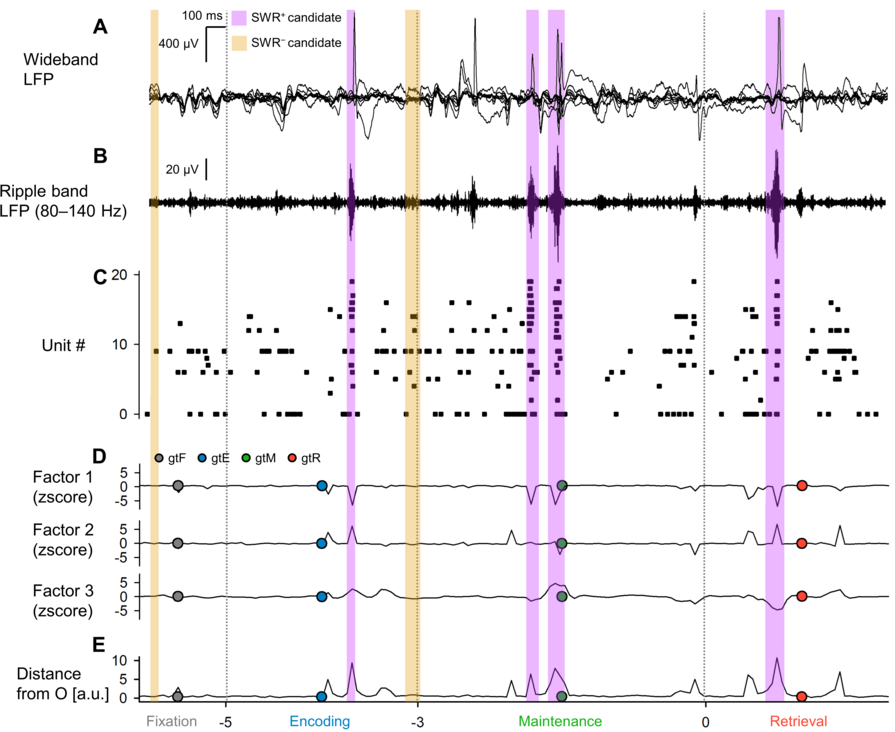
\includegraphics[width=1\textwidth]{./src/figures/.png/Figure_ID_01.png}
        	\caption{\textbf{
Local Field Potentials (LFP), Multiunit Activity, and Neural Trajectories in the Hippocampus During a Modified Sternberg Task
}
\smallskip
\\
\textbf{\textit{A.}} Representative wideband LFP signals for intracranial EEG recording from the left hippocampal head \DIFaddbeginFL \DIFaddFL{are presented}\DIFaddendFL . \DIFdelbeginFL \DIFdelFL{The }\DIFdelendFL \DIFaddbeginFL \DIFaddFL{This recording took place while the }\DIFaddendFL subject performed a modified Sternberg working memory task\DIFdelbeginFL \DIFdelFL{, which includes }\DIFdelendFL \DIFaddbeginFL \DIFaddFL{. Task stages included }\DIFaddendFL fixation (1 s, \textit{gray}), encoding (2 s, \textit{blue}), maintenance (3 s, \textit{green}), and retrieval (2 s, \textit{red}). \textbf{\textit{B.}} \DIFdelbeginFL \DIFdelFL{The corresponding }\DIFdelendFL \DIFaddbeginFL \DIFaddFL{Displays the associated }\DIFaddendFL ripple band LFP traces. Note \DIFdelbeginFL \DIFdelFL{that }\DIFdelendFL \textit{purple} and \textit{yellow} rectangles\DIFdelbeginFL \DIFdelFL{indicating }\DIFdelendFL \DIFaddbeginFL \DIFaddFL{, which denote }\DIFaddendFL the timings for SWR$^+$ candidates and SWR$^-$ candidates\DIFaddbeginFL \DIFaddFL{, respectively }\DIFaddendFL (\DIFaddbeginFL \DIFaddFL{the latter serving as }\DIFaddendFL control events for SWR$^+$)\DIFdelbeginFL \DIFdelFL{, respectively}\DIFdelendFL . \textbf{\textit{C.}} \DIFdelbeginFL \DIFdelFL{The }\DIFdelendFL \DIFaddbeginFL \DIFaddFL{A }\DIFaddendFL raster plot \DIFdelbeginFL \DIFdelFL{depicts }\DIFdelendFL \DIFaddbeginFL \DIFaddFL{illustrates }\DIFaddendFL multiunit spikes \DIFdelbeginFL \DIFdelFL{taken }\DIFdelendFL from the LFP traces\DIFdelbeginFL \DIFdelFL{, }\DIFdelendFL \DIFaddbeginFL \DIFaddFL{. These spikes have been }\DIFaddendFL sorted using a spike algorithm \cite{niediek_reliable_2016}. \textbf{\textit{D.}} \DIFdelbeginFL \DIFdelFL{Neural }\DIFdelendFL \DIFaddbeginFL \DIFaddFL{Shows neural }\DIFaddendFL trajectories \DIFdelbeginFL \DIFdelFL{calculated }\DIFdelendFL \DIFaddbeginFL \DIFaddFL{computed }\DIFaddendFL by GPFA\cite{yu_gaussian-process_2009} \DIFaddbeginFL \DIFaddFL{based }\DIFaddendFL on spike counts per unit with 50-ms bins. \DIFdelbeginFL \DIFdelFL{Each phase's }\DIFdelendFL \DIFaddbeginFL \DIFaddFL{The }\DIFaddendFL geometric median \DIFaddbeginFL \DIFaddFL{of each phase }\DIFaddendFL is marked by \DIFdelbeginFL \DIFdelFL{the }\DIFdelendFL dot circles. \textbf{\textit{E.}} \DIFdelbeginFL \DIFdelFL{The }\DIFdelendFL \DIFaddbeginFL \DIFaddFL{Indicates the }\DIFaddendFL distance of \DIFaddbeginFL \DIFaddFL{the }\DIFaddendFL neural trajectory from the origin \DIFaddbeginFL \DIFaddFL{point }\DIFaddendFL $O$.
}
% width=1\textwidth
        	\label{fig:01}
        \end{figure*}
        \clearpage
        \begin{figure*}[ht]
            \pdfbookmark[2]{ID 02}{figure_id_02}
        	\centering
            \includegraphics[width=0.5\textwidth]{./src/figures/.png/Figure_ID_02.png}
        	\caption{\textbf{
State-Dependent Trajectories of Hippocampal Neurons
}
\smallskip
\\
\textbf{\textit{A.}} Neural trajectories \DIFaddbeginFL \DIFaddFL{are depicted }\DIFaddendFL as a point cloud within the \DIFdelbeginFL \DIFdelFL{initial }\DIFdelendFL \DIFaddbeginFL \DIFaddFL{first }\DIFaddendFL three-dimensional factors derived from \DIFaddbeginFL \DIFaddFL{Gaussian Process Factor Analysis (}\DIFaddendFL GPFA\DIFaddbeginFL \DIFaddFL{) }\DIFaddendFL \cite{yu_gaussian-process_2009}. The smaller dots \DIFdelbeginFL \DIFdelFL{correspond to coordinates of }\DIFdelendFL \DIFaddbeginFL \DIFaddFL{represent }\DIFaddendFL 50-ms neural trajectory bins, \DIFdelbeginFL \DIFdelFL{while }\DIFdelendFL \DIFaddbeginFL \DIFaddFL{and }\DIFaddendFL the larger dots with \textit{black} edges \DIFdelbeginFL \DIFdelFL{show }\DIFdelendFL \DIFaddbeginFL \DIFaddFL{denote }\DIFaddendFL the geometric medians for \DIFdelbeginFL \DIFdelFL{respective phases }\DIFdelendFL \DIFaddbeginFL \DIFaddFL{each phase }\DIFaddendFL in the Sternberg working memory task: fixation ($\mathrm{\lVert g_{F} \rVert}$, \textit{gray}), encoding ($\mathrm{\lVert g_{E} \rVert}$, \textit{blue}), maintenance ($\mathrm{\lVert g_{M} \rVert}$, \textit{green}), and retrieval ($\mathrm{\lVert g_{R} \rVert}$, \textit{red}). \textbf{\textit{B.}} The figure \DIFdelbeginFL \DIFdelFL{conveys }\DIFdelendFL \DIFaddbeginFL \DIFaddFL{presents }\DIFaddendFL the log-likelihood of the GPFA models versus the \DIFdelbeginFL \DIFdelFL{count }\DIFdelendFL \DIFaddbeginFL \DIFaddFL{number }\DIFaddendFL of dimensions used to embed multiunit spikes found in the medial temporal lobe (MTL) \DIFdelbeginFL \DIFdelFL{territories}\DIFdelendFL \DIFaddbeginFL \DIFaddFL{regions}\DIFaddendFL . \DIFdelbeginFL \DIFdelFL{In specific}\DIFdelendFL \DIFaddbeginFL \DIFaddFL{Specifically}\DIFaddendFL , the elbow method \DIFdelbeginFL \DIFdelFL{pinpointed }\DIFdelendFL \DIFaddbeginFL \DIFaddFL{identified three as }\DIFaddendFL the optimal dimension\DIFdelbeginFL \DIFdelFL{to be three}\DIFdelendFL . \textbf{\textit{C.}} This panel \DIFdelbeginFL \DIFdelFL{illustrates }\DIFdelendFL \DIFaddbeginFL \DIFaddFL{displays }\DIFaddendFL the distance of the neural trajectories from the origin ($O$) for the hippocampus (Hipp.), entorhinal cortex (EC), and amygdala (Amy.), \DIFaddbeginFL \DIFaddFL{plotted }\DIFaddendFL against the time elapsed from the probe onset. \textbf{\textit{D.}} The \DIFdelbeginFL \DIFdelFL{distance of the }\DIFdelendFL trajectory \DIFaddbeginFL \DIFaddFL{distance }\DIFaddendFL from $O$ within \DIFaddbeginFL \DIFaddFL{the }\DIFaddendFL MTL regions is \DIFdelbeginFL \DIFdelFL{displayed}\DIFdelendFL \DIFaddbeginFL \DIFaddFL{shown}\DIFaddendFL . The hippocampus \DIFdelbeginFL \DIFdelFL{shows }\DIFdelendFL \DIFaddbeginFL \DIFaddFL{has }\DIFaddendFL the \DIFdelbeginFL \DIFdelFL{farthest }\DIFdelendFL \DIFaddbeginFL \DIFaddFL{greatest }\DIFaddendFL distance, followed by the EC and the Amygdala. \textbf{\textit{E.}} The box plot \DIFdelbeginFL \DIFdelFL{represents }\DIFdelendFL \DIFaddbeginFL \DIFaddFL{illustrates }\DIFaddendFL inter-phase trajectory distances within the MTL regions.
}
% width=0.5\textwidth
        	\label{fig:02}
        \end{figure*}
        \clearpage
        \begin{figure*}[ht]
            \pdfbookmark[2]{ID 03}{figure_id_03}
        	\centering
            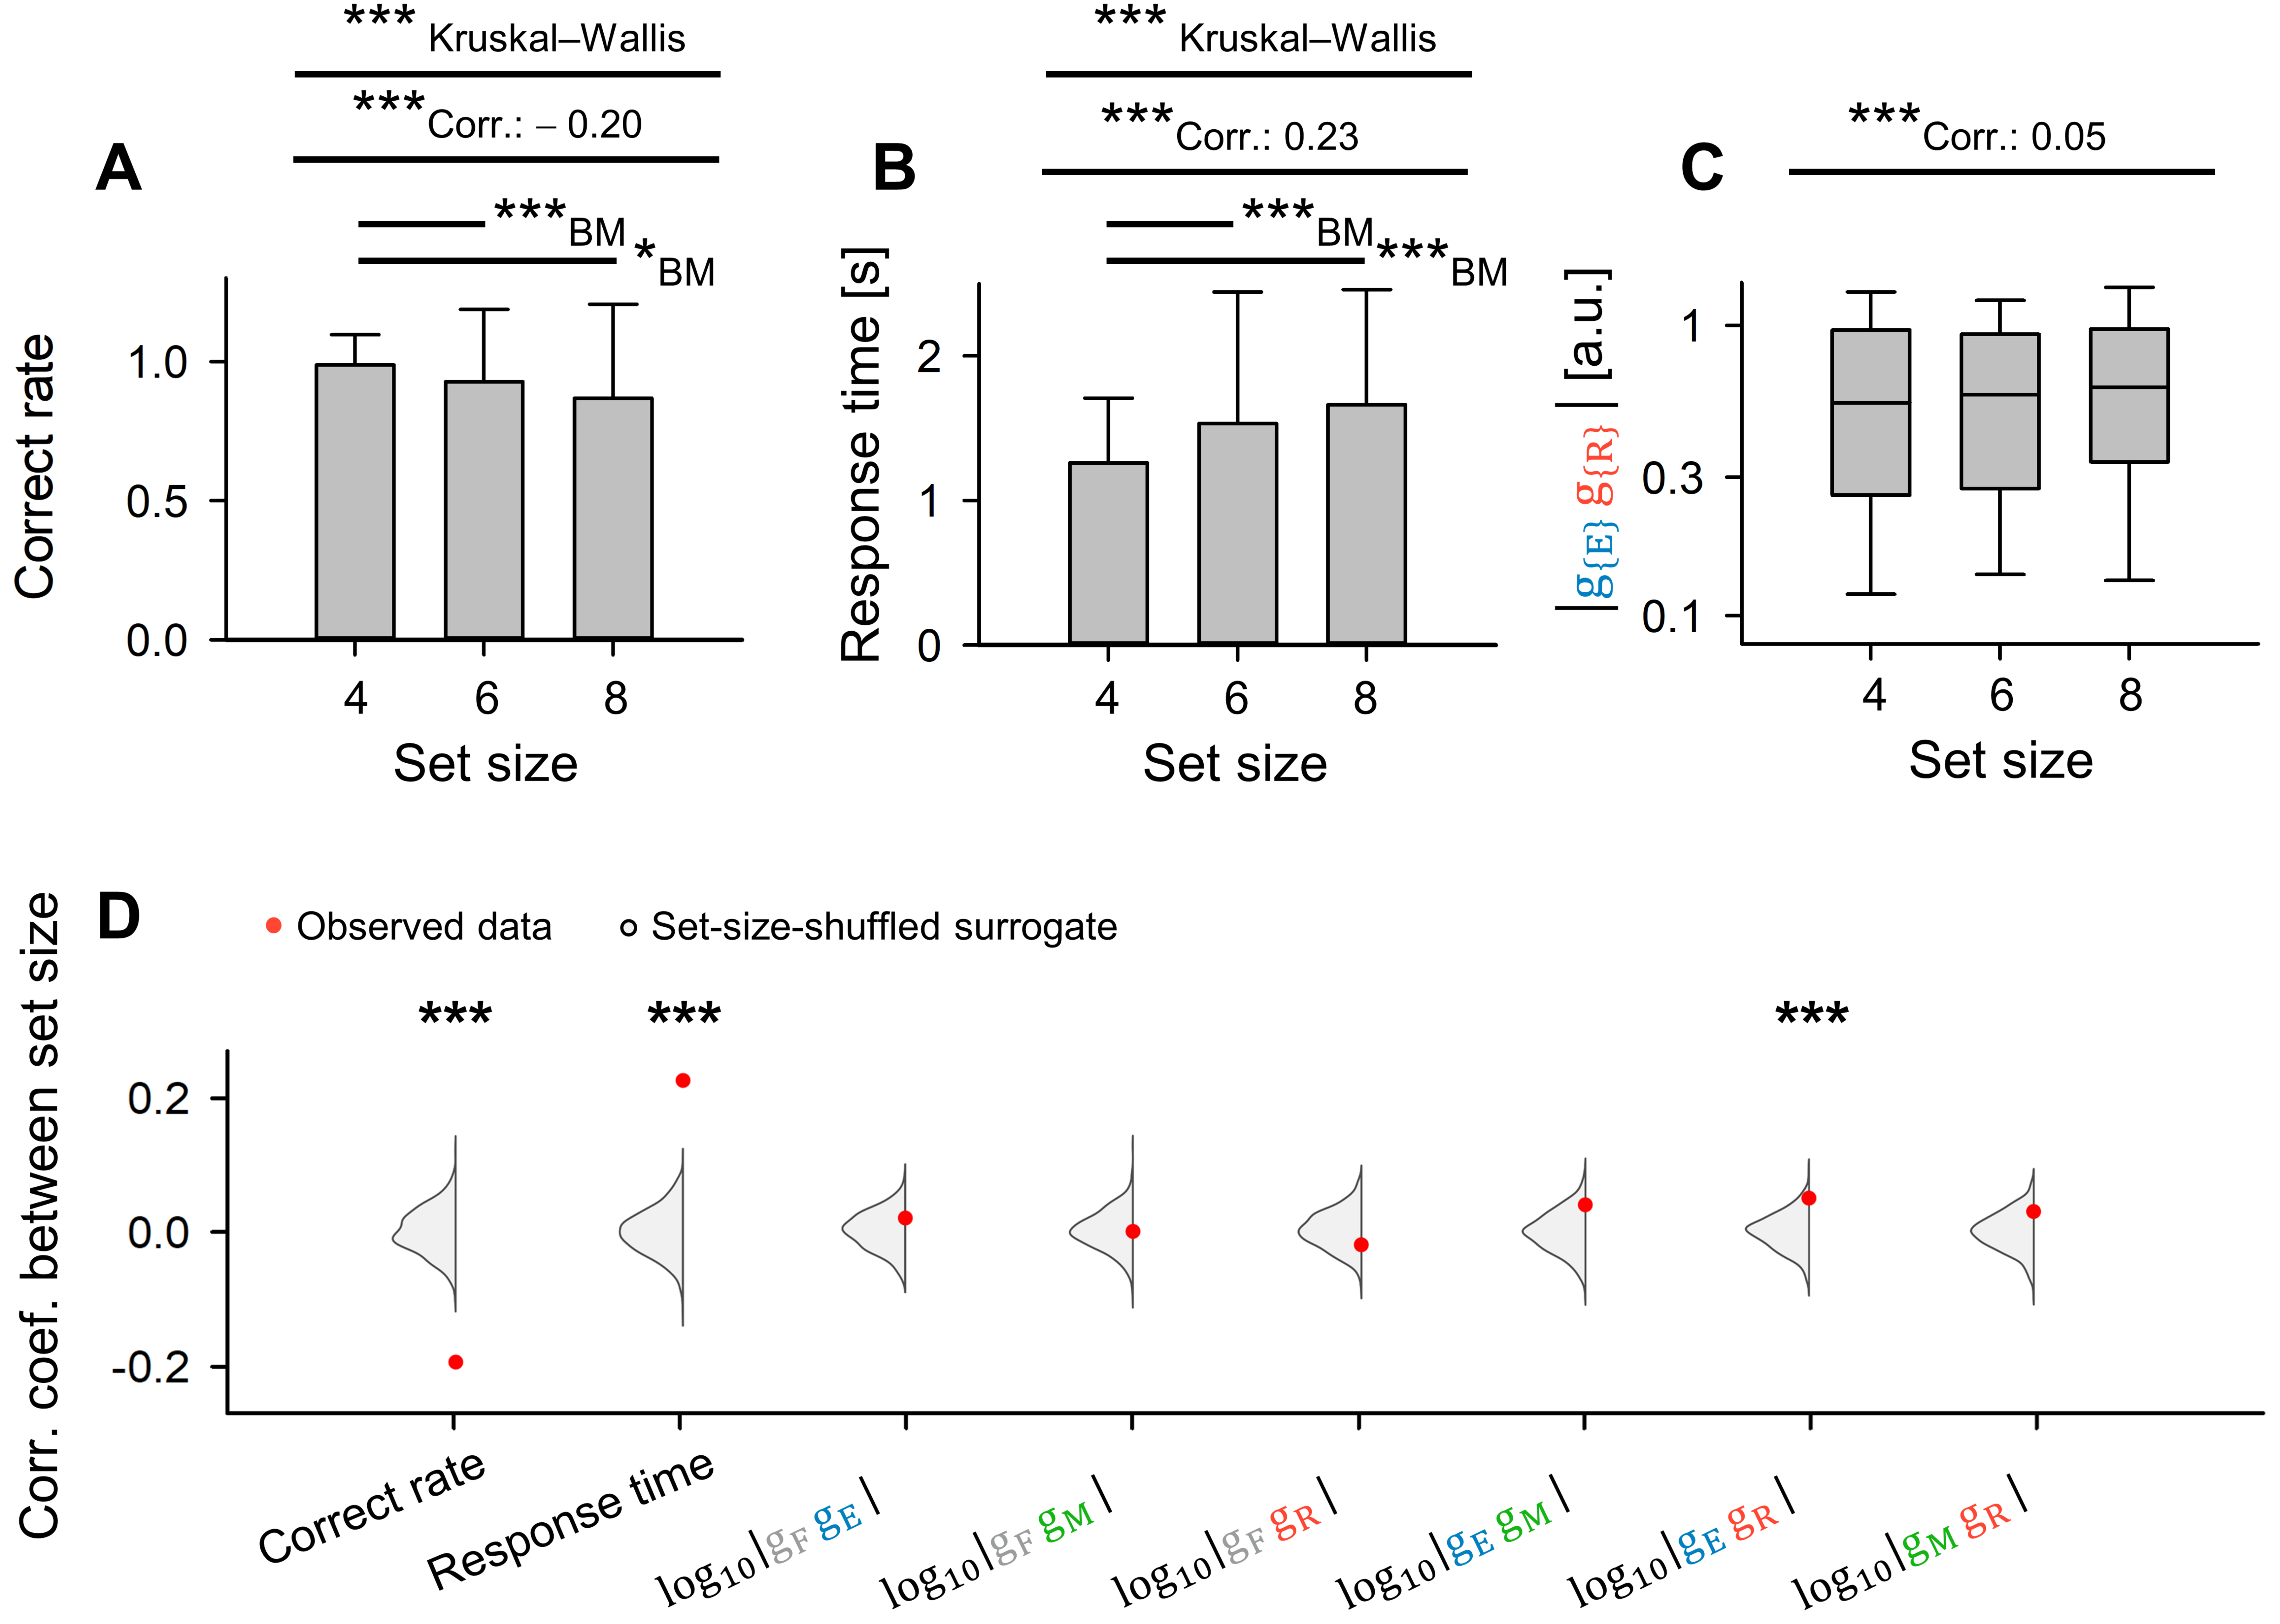
\includegraphics[width=1\textwidth]{./src/figures/.png/Figure_ID_03.png}
        	\caption{\DIFdelbeginFL \textbf{\DIFdelFL{Dependency of Trajectory Distance on Memory Load: Encoding and Retrieval States in Hippocampus
}}
%DIFAUXCMD
\DIFdelendFL \DIFaddbeginFL \textbf{
\DIFaddFL{Relationship between Trajectory Distance and Memory Load: States of Encoding and Retrieval in the Hippocampus
}}
\DIFaddendFL \smallskip
\\
\textbf{\textit{A.}} \DIFdelbeginFL \DIFdelFL{The }\DIFdelendFL \DIFaddbeginFL \DIFaddFL{Demonstrates the }\DIFaddendFL relationship between set size (number of letters \DIFdelbeginFL \DIFdelFL{that need }\DIFdelendFL to be encoded) and \DIFdelbeginFL \DIFdelFL{correct rate }\DIFdelendFL \DIFaddbeginFL \DIFaddFL{accuracy }\DIFaddendFL in the working memory task (coefficient = $-0.20$, ***\textit{p} $<$ 0.001). \textbf{\textit{B.}} \DIFdelbeginFL \DIFdelFL{The }\DIFdelendFL \DIFaddbeginFL \DIFaddFL{Displays the }\DIFaddendFL correlation between set size and response time (coefficient = 0.23, ***\textit{p} $<$ 0.001). \textbf{\textit{C.}} \DIFdelbeginFL \DIFdelFL{The impact }\DIFdelendFL \DIFaddbeginFL \DIFaddFL{Exhibits the influence }\DIFaddendFL of set size on the inter-phase distances between the encoding and retrieval phases ($\lVert \mathrm{g_{E}g_{R}} \rVert$) (correlation coefficient = 0.05, ***\textit{p} $<$ 0.001). \textbf{\textit{D.}} \DIFdelbeginFL \textit{\DIFdelFL{Red}} %DIFAUXCMD
\DIFdelFL{dots represent }\DIFdelendFL \DIFaddbeginFL \DIFaddFL{Indicates }\DIFaddendFL experimental observations of correlations between set size and the following parameters: \DIFdelbeginFL \DIFdelFL{correct rate}\DIFdelendFL \DIFaddbeginFL \DIFaddFL{accuracy}\DIFaddendFL , response time, $\log_{10}{\lVert \mathrm{g_{F}g_{E}} \rVert}$, $\log_{10}{\lVert \mathrm{g_{F}g_{M}} \rVert}$, $\log_{10}{\lVert \mathrm{g_{F}g_{R}} \rVert}$, $\log_{10}{\lVert \mathrm{g_{E}g_{M}} \rVert}$, $\log_{10}{\lVert \mathrm{g_{E}g_{R}} \rVert}$, and $\log_{10}{\lVert \mathrm{g_{M}g_{R}} \rVert}$ \DIFaddbeginFL \DIFaddFL{represented by }\textit{\DIFaddFL{red}} \DIFaddFL{dots}\DIFaddendFL . The \textit{gray} kernel density plots illustrate the corresponding \DIFdelbeginFL \DIFdelFL{set-size-shuffled }\DIFdelendFL \DIFaddbeginFL \DIFaddFL{shuffled }\DIFaddendFL surrogate \DIFaddbeginFL \DIFaddFL{with set size }\DIFaddendFL (\textit{n} = 1,000) (***\textit{p}s $<$ 0.001).
}
% width=1\textwidth
        	\label{fig:03}
        \end{figure*}
        \clearpage
        \begin{figure*}[ht]
            \pdfbookmark[2]{ID 04}{figure_id_04}
        	\centering
            \DIFdelbeginFL %DIFDELCMD < \includegraphics[width=1\textwidth]{./src/figures/.png/Figure_ID_04.png}
%DIFDELCMD <         	%%%
\DIFdelendFL \DIFaddbeginFL \includegraphics[width=]{./src/figures/.png/Figure_ID_04.png}
        	\DIFaddendFL \caption{\DIFdelbeginFL \textbf{\DIFdelFL{Detection of SWRs in Presumptive CA1 Regions
}}
%DIFAUXCMD
%DIFDELCMD < \smallskip
%DIFDELCMD < %%%
\DIFdelendFL \DIFaddbeginFL \textbf{\DIFaddFL{Detection of SWRs in Presumptive CA1 Regions}}\DIFaddendFL \\
\textbf{\textit{A.}} Two-dimensional UMAP \cite{mcinnes_umap_2018} projection \DIFdelbeginFL \DIFdelFL{of multiunit }\DIFdelendFL \DIFaddbeginFL \DIFaddFL{displays multi-unit }\DIFaddendFL spikes during SWR$^+$ candidates (\textit{purple}) and SWR$^-$ candidates (\textit{yellow}). \textbf{\textit{B.}} \DIFdelbeginFL \DIFdelFL{Cumulative }\DIFdelendFL \DIFaddbeginFL \DIFaddFL{A cumulative }\DIFaddendFL density plot \DIFdelbeginFL \DIFdelFL{showing }\DIFdelendFL \DIFaddbeginFL \DIFaddFL{indicates }\DIFaddendFL silhouette scores, \DIFdelbeginFL \DIFdelFL{indicative of }\DIFdelendFL \DIFaddbeginFL \DIFaddFL{reflecting }\DIFaddendFL UMAP clustering quality (see Table~\ref{tab:02}). \DIFdelbeginFL \DIFdelFL{Note that hippocampal }\DIFdelendFL \DIFaddbeginFL \DIFaddFL{Hippocampal }\DIFaddendFL regions with silhouette scores \DIFdelbeginFL \DIFdelFL{greater than }\DIFdelendFL \DIFaddbeginFL \DIFaddFL{exceeding }\DIFaddendFL 0.60 (equivalent to the $75^{th}$ percentile) \DIFdelbeginFL \DIFdelFL{were defined }\DIFdelendFL \DIFaddbeginFL \DIFaddFL{are identified }\DIFaddendFL as putative CA1 regions. SWR$^+$ and SWR$^-$ candidates\DIFaddbeginFL \DIFaddFL{, which were }\DIFaddendFL recorded from these \DIFdelbeginFL \DIFdelFL{putative CA1 }\DIFdelendFL regions\DIFdelbeginFL \DIFdelFL{were respectively }\DIFdelendFL \DIFaddbeginFL \DIFaddFL{, are }\DIFaddendFL classified as SWR$^+$ and SWR$^-$ \DIFaddbeginFL \DIFaddFL{respectively }\DIFaddendFL (\textit{n}s = 1,170). \textbf{\textit{C.}} \DIFdelbeginFL \DIFdelFL{The identical }\DIFdelendFL \DIFaddbeginFL \DIFaddFL{Identical }\DIFaddendFL distributions of durations are presented for SWR$^+$ (\textit{purple}) and SWR$^-$ (\textit{yellow}), \DIFdelbeginFL \DIFdelFL{owing to }\DIFdelendFL \DIFaddbeginFL \DIFaddFL{based on }\DIFaddendFL their definitions (93.0 [65.4] ms, median [IQR]). \textbf{\textit{D.}} SWR incidence for both SWR$^+$ (\textit{purple}) and SWR$^-$ (\textit{yellow})\DIFdelbeginFL \DIFdelFL{obtained }\DIFdelendFL \DIFaddbeginFL \DIFaddFL{, }\DIFaddendFL relative to the probe's timing\DIFaddbeginFL \DIFaddFL{, }\DIFaddendFL is illustrated as a mean \textpm 95\% confidence interval. However, \DIFdelbeginFL \DIFdelFL{as the }\DIFdelendFL intervals may not be \DIFdelbeginFL \DIFdelFL{visible }\DIFdelendFL \DIFaddbeginFL \DIFaddFL{visibly apparent }\DIFaddendFL due to their \DIFdelbeginFL \DIFdelFL{narrow }\DIFdelendFL \DIFaddbeginFL \DIFaddFL{confined }\DIFaddendFL ranges, \DIFdelbeginFL \DIFdelFL{note }\DIFdelendFL \DIFaddbeginFL \DIFaddFL{be aware }\DIFaddendFL that a significant \DIFdelbeginFL \DIFdelFL{increase in }\DIFdelendFL SWR incidence \DIFaddbeginFL \DIFaddFL{increase }\DIFaddendFL was detected during the initial 400 ms of the retrieval phase (0.421 [Hz], *\textit{p} $<$ 0.05, bootstrap test). \textbf{\textit{E.}} \DIFdelbeginFL \DIFdelFL{The distributions }\DIFdelendFL \DIFaddbeginFL \DIFaddFL{Distributions }\DIFaddendFL of ripple band peak amplitudes for SWR$^-$ (\textit{yellow}; 2.37 [0.33] SD of baseline, median [IQR]) and SWR$^+$ (\textit{purple}; 3.05 [0.85] SD of baseline, median [IQR]) are \DIFdelbeginFL \DIFdelFL{delineated }\DIFdelendFL \DIFaddbeginFL \DIFaddFL{manifested }\DIFaddendFL (***\textit{p} $<$ 0.001, the Brunner--Munzel test).}
        	%DIF <  width=1\textwidth
        	\label{fig:04}
        \end{figure*}
        \clearpage
        \begin{figure*}[ht]
            \pdfbookmark[2]{ID 05}{figure_id_05}
        	\centering
            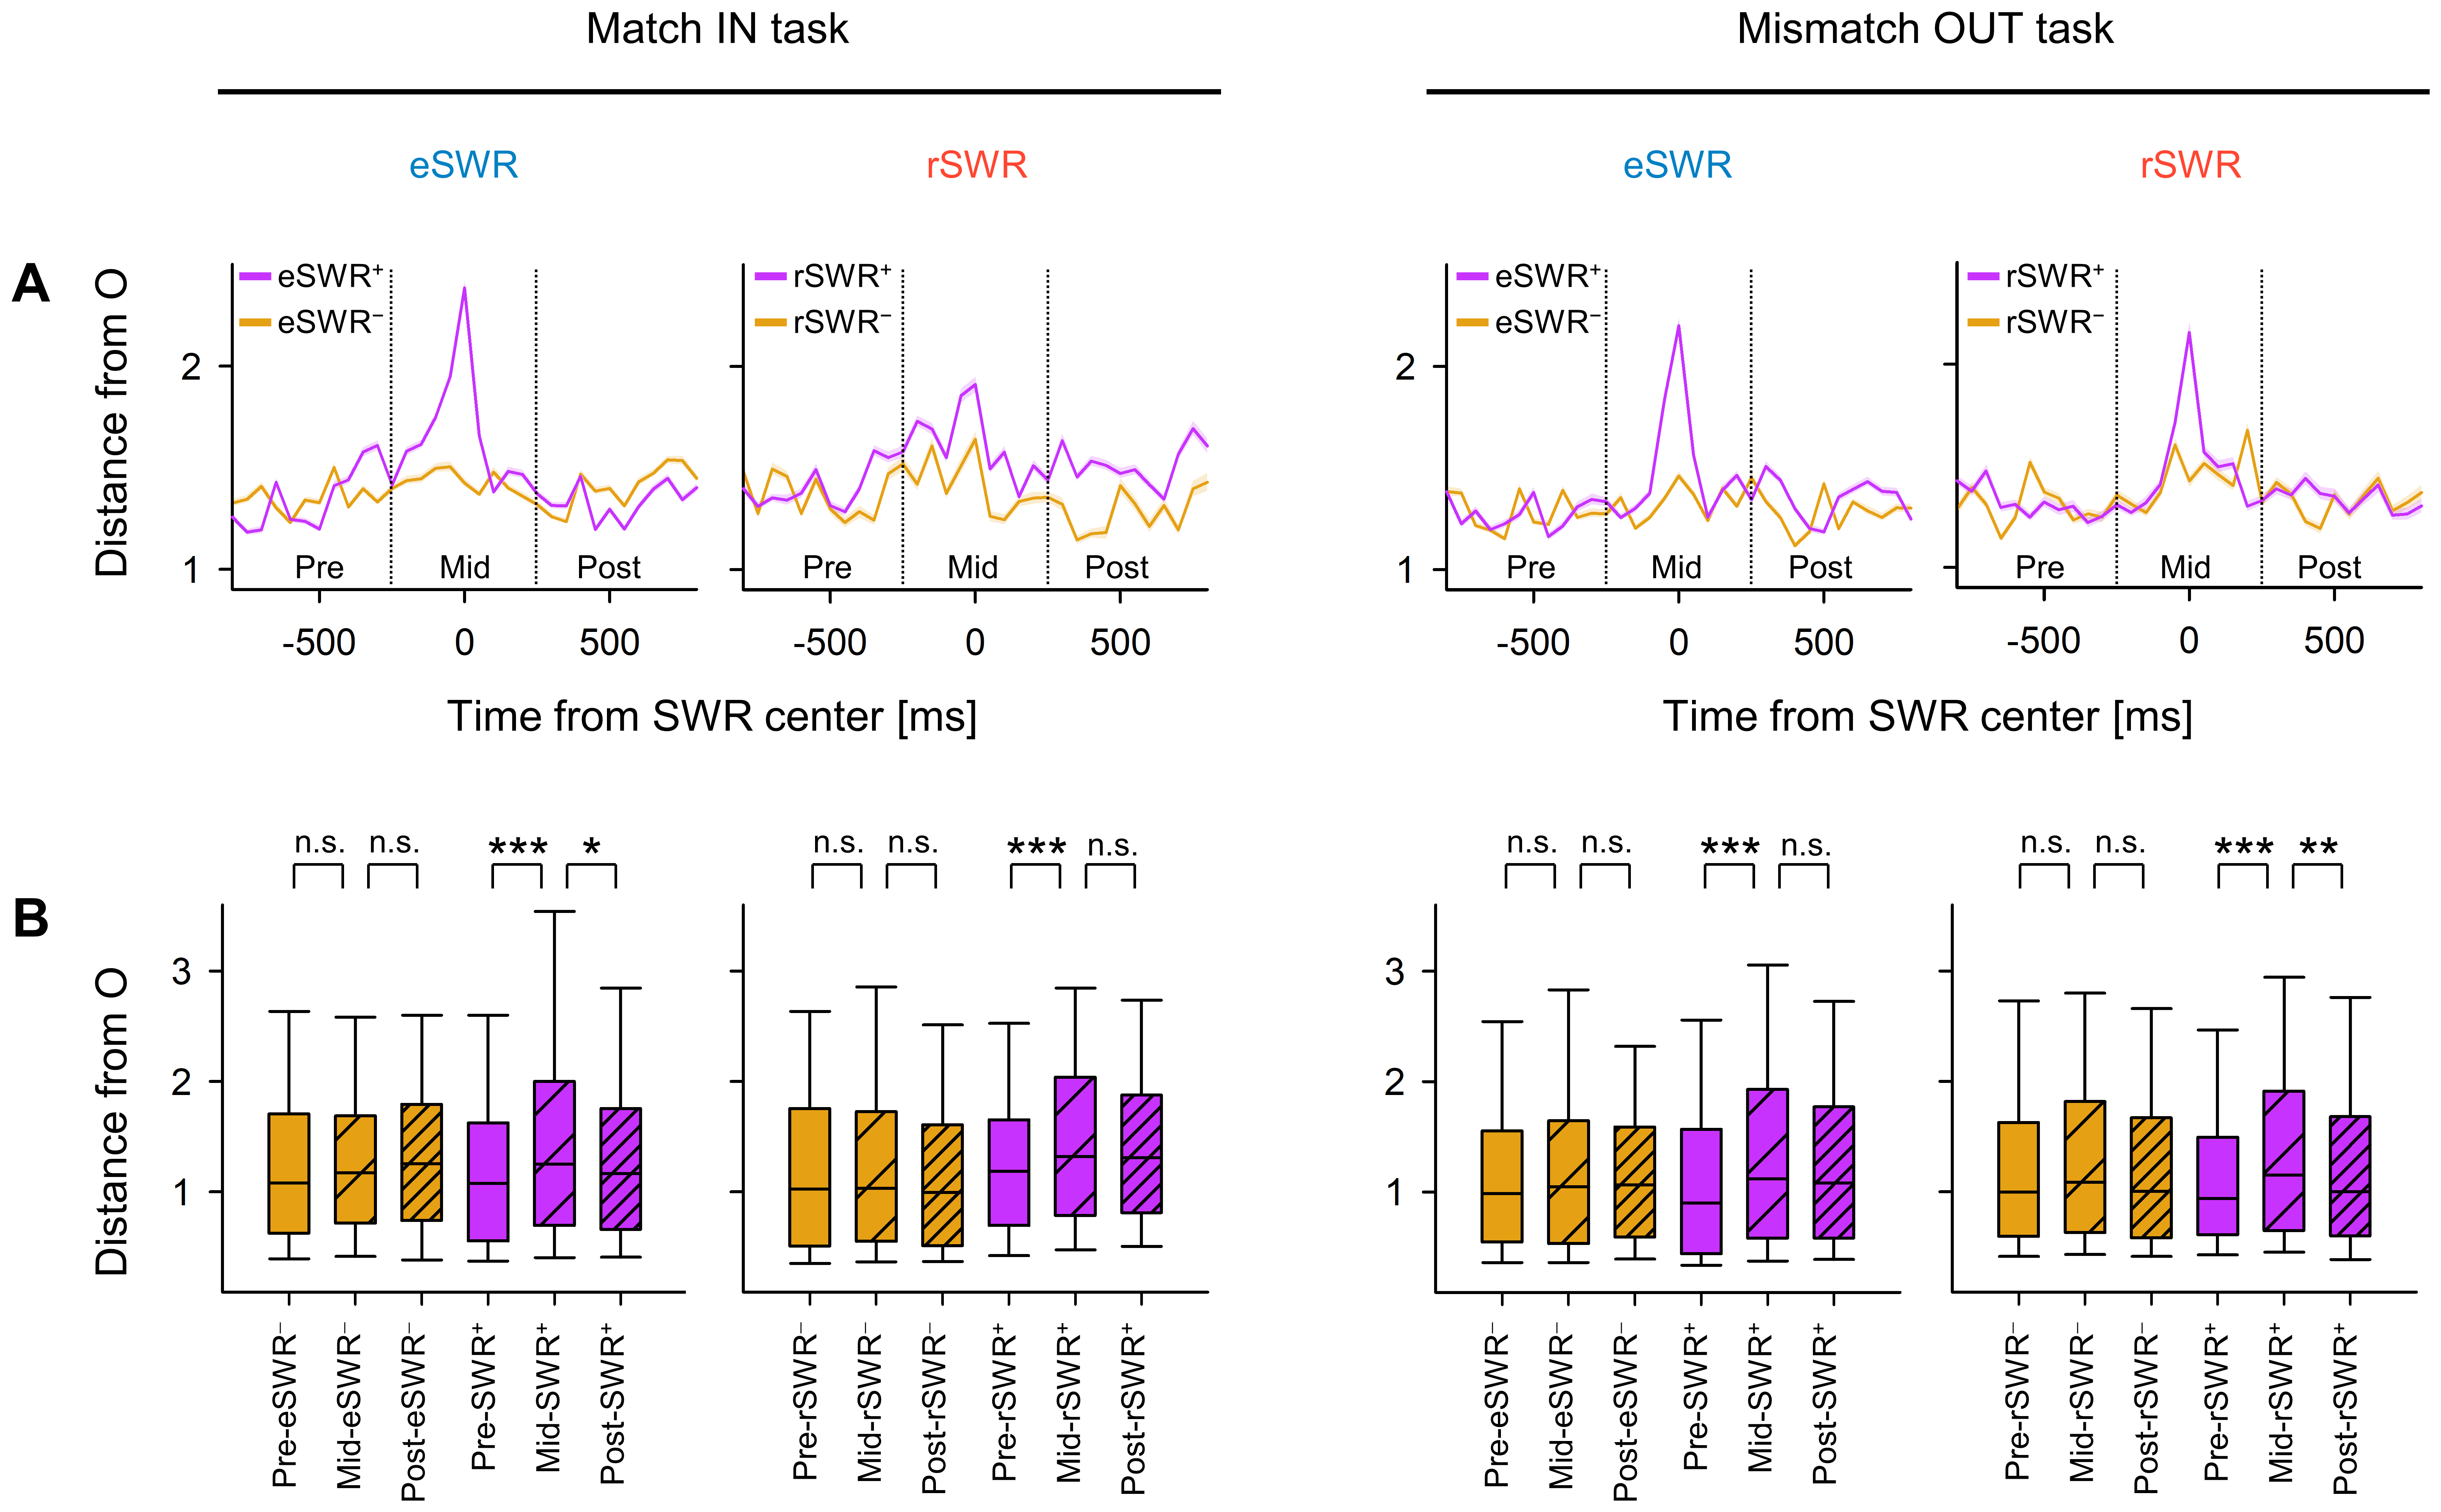
\includegraphics[width=1\textwidth]{./src/figures/.png/Figure_ID_05.png}
        	\caption{\DIFdelbeginFL \textbf{\DIFdelFL{Transient Alterations in Neural Trajectory During SWR Events
}}
%DIFAUXCMD
\DIFdelendFL \DIFaddbeginFL \textbf{\DIFaddFL{Transient Changes in Neural Pathway During SWR Events}}
\DIFaddendFL \smallskip
\\
\textbf{\textit{A.}} \DIFdelbeginFL \DIFdelFL{Displayed }\DIFdelendFL \DIFaddbeginFL \DIFaddFL{Presented }\DIFaddendFL is the distance from origin ($O$) of the peri-sharp-wave-ripple \DIFdelbeginFL \DIFdelFL{trajectory }\DIFdelendFL \DIFaddbeginFL \DIFaddFL{pathway }\DIFaddendFL (mean \textpm 95\% confidence interval). The intervals may \DIFdelbeginFL \DIFdelFL{not }\DIFdelendFL be \DIFdelbeginFL \DIFdelFL{apparent }\DIFdelendFL \DIFaddbeginFL \DIFaddFL{obscured }\DIFaddendFL due to their \DIFdelbeginFL \DIFdelFL{narrow }\DIFdelendFL \DIFaddbeginFL \DIFaddFL{minimal }\DIFaddendFL ranges. \textbf{\textit{B.}} \DIFdelbeginFL \DIFdelFL{Shown is the }\DIFdelendFL \DIFaddbeginFL \DIFaddFL{The }\DIFaddendFL distance from the origin ($O$) during \DIFaddbeginFL \DIFaddFL{the }\DIFaddendFL pre-, mid-, and post-SWR periods \DIFaddbeginFL \DIFaddFL{is demonstrated }\DIFaddendFL (*\textit{p} $<$ 0.05, **\textit{p} $<$ 0.01, ***\textit{p} $<$ 0.001; \DIFdelbeginFL \DIFdelFL{the }\DIFdelendFL Brunner--Munzel test \DIFaddbeginFL \DIFaddFL{applied}\DIFaddendFL ). Abbreviations: SWR, sharp-wave ripple events; eSWR, SWR during the encoding phase; rSWR, SWR \DIFdelbeginFL \DIFdelFL{while in }\DIFdelendFL \DIFaddbeginFL \DIFaddFL{within }\DIFaddendFL the retrieval phase; SWR$^+$, positive SWR event; SWR$^-$, control events for SWR$^+$; pre-, mid-, or post-SWR \DIFdelbeginFL \DIFdelFL{denote }\DIFdelendFL \DIFaddbeginFL \DIFaddFL{refer to }\DIFaddendFL the time intervals from $-800$ to $-250$ ms, from $-250$ to $+250$ ms, or from $+250$ to $+800$ ms, \DIFaddbeginFL \DIFaddFL{respectively, }\DIFaddendFL all relative to the \DIFdelbeginFL \DIFdelFL{center of the }\DIFdelendFL SWR \DIFaddbeginFL \DIFaddFL{center}\DIFaddendFL .}
% width=1\textwidth
        	\label{fig:05}
        \end{figure*}
        \clearpage
        \begin{figure*}[ht]
            \pdfbookmark[2]{ID 06}{figure_id_06}
        	\centering
            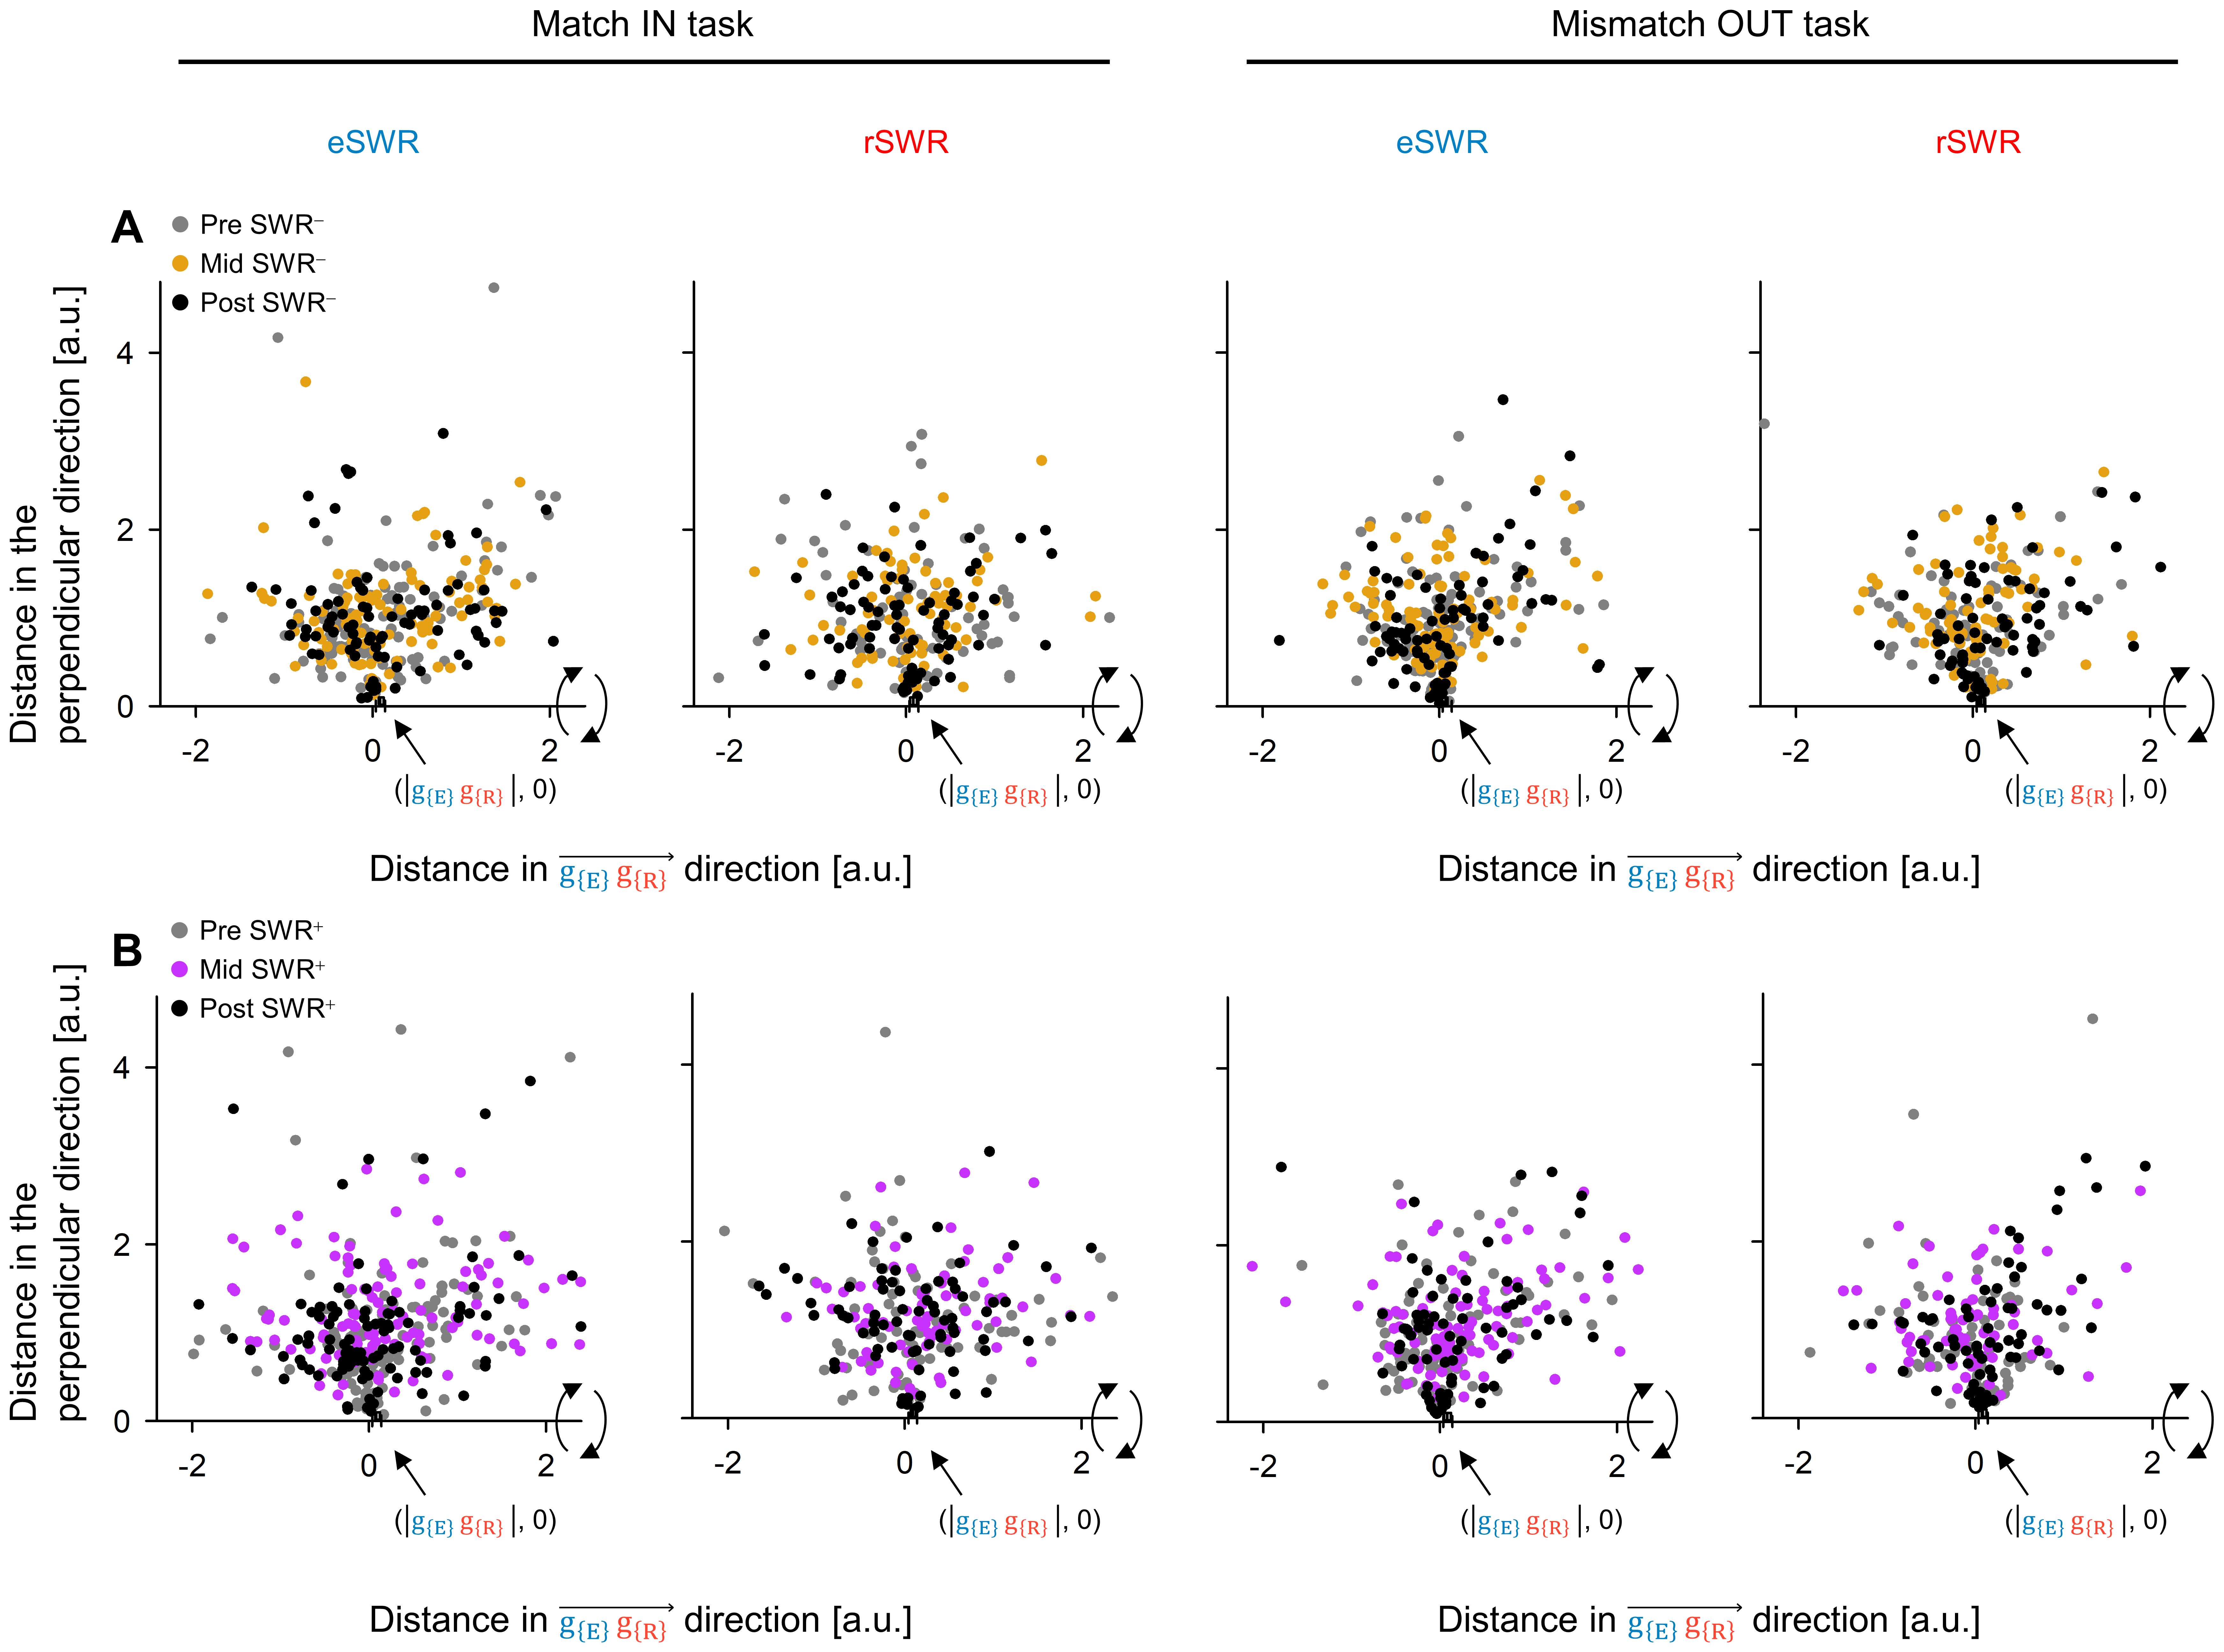
\includegraphics[width=1\textwidth]{./src/figures/.png/Figure_ID_06.png}
        	\caption{\textbf{
Visualization of Neural Trajectories during SWR in Two-Dimensional Spaces}
\smallskip
\\
The panels \DIFdelbeginFL \DIFdelFL{display }\DIFdelendFL \DIFaddbeginFL \DIFaddFL{depict }\DIFaddendFL hippocampal neural trajectories during SWR \DIFdelbeginFL \DIFdelFL{as }\DIFdelendFL projected onto two-dimensional spaces. \textbf{\textit{A.}} \DIFdelbeginFL \DIFdelFL{Hippocampal }\DIFdelendFL \DIFaddbeginFL \DIFaddFL{Shows the hippocampal }\DIFaddendFL neural trajectories as point clouds during pre-SWR$^-$ (\textit{gray}), mid-SWR$^-$ (\textit{yellow}), and post-SWR$^-$ (\textit{black}). \textbf{\textit{B.}} \DIFdelbeginFL \DIFdelFL{Represents }\DIFdelendFL \DIFaddbeginFL \DIFaddFL{Conveys }\DIFaddendFL the \DIFdelbeginFL \DIFdelFL{equivalents }\DIFdelendFL \DIFaddbeginFL \DIFaddFL{equivalent }\DIFaddendFL for SWR$^+$ \DIFdelbeginFL \DIFdelFL{as opposed to }\DIFdelendFL \DIFaddbeginFL \DIFaddFL{rather than }\DIFaddendFL SWR$^-$. The projection was \DIFdelbeginFL \DIFdelFL{applied in the following manner}\DIFdelendFL \DIFaddbeginFL \DIFaddFL{executed as follows}\DIFaddendFL : First, a linear transformation \DIFdelbeginFL \DIFdelFL{positioned }\DIFdelendFL \DIFaddbeginFL \DIFaddFL{placed }\DIFaddendFL $\mathrm{g_{E}}$ at the origin $O$ (0,0), and $\mathrm{g_{R}}$ at ($\lVert \mathrm{g_{E}g_{R}} \rVert$, 0). The point cloud was \DIFdelbeginFL \DIFdelFL{then }\DIFdelendFL \DIFaddbeginFL \DIFaddFL{subsequently }\DIFaddendFL rotated around the $\mathrm{g_{E}g_{R}}$ axis (\DIFdelbeginFL \DIFdelFL{equivalent }\DIFdelendFL \DIFaddbeginFL \DIFaddFL{similar }\DIFaddendFL to the x axis) for \DIFdelbeginFL \DIFdelFL{fitting into }\DIFdelendFL \DIFaddbeginFL \DIFaddFL{adaptation to }\DIFaddendFL two-dimensional spaces. \DIFdelbeginFL \DIFdelFL{Therefore}\DIFdelendFL \DIFaddbeginFL \DIFaddFL{Thus}\DIFaddendFL , within these two-dimensional spaces, \DIFdelbeginFL \DIFdelFL{both }\DIFdelendFL the distances from \DIFaddbeginFL \DIFaddFL{point }\DIFaddendFL $O$ and the angles for the $\mathrm{g_{E}g_{R}}$ axis are \DIFdelbeginFL \DIFdelFL{preserved }\DIFdelendFL \DIFaddbeginFL \DIFaddFL{retained as in }\DIFaddendFL the original \DIFdelbeginFL \DIFdelFL{three dimensional }\DIFdelendFL \DIFaddbeginFL \DIFaddFL{three-dimensional }\DIFaddendFL spaces \DIFdelbeginFL \DIFdelFL{in }\DIFdelendFL \DIFaddbeginFL \DIFaddFL{created by }\DIFaddendFL GPFA. Abbreviations: SWR \DIFdelbeginFL \DIFdelFL{signifies }\DIFdelendFL \DIFaddbeginFL \DIFaddFL{denotes }\DIFaddendFL sharp-wave ripple events; eSWR \DIFdelbeginFL \DIFdelFL{denotes }\DIFdelendFL \DIFaddbeginFL \DIFaddFL{refers to }\DIFaddendFL SWR during the encoding phase; rSWR \DIFdelbeginFL \DIFdelFL{indicates }\DIFdelendFL \DIFaddbeginFL \DIFaddFL{signals }\DIFaddendFL SWR during the retrieval phase; SWR$^+$, \DIFdelbeginFL \DIFdelFL{marks }\DIFdelendFL \DIFaddbeginFL \DIFaddFL{characterizes }\DIFaddendFL an SWR event; SWR$^-$ \DIFdelbeginFL \DIFdelFL{refers to }\DIFdelendFL \DIFaddbeginFL \DIFaddFL{signifies }\DIFaddendFL control events for SWR$^+$; pre-SWR, mid-SWR, or post-SWR, \DIFdelbeginFL \DIFdelFL{reference }\DIFdelendFL \DIFaddbeginFL \DIFaddFL{represent }\DIFaddendFL the time intervals from $-800$ to $-250$ ms, from $-250$ to $+250$ ms, or from $+250$ to $+800$ ms from the center of \DIFaddbeginFL \DIFaddFL{the }\DIFaddendFL SWR.
}
% width=1\textwidth
        	\label{fig:06}
        \end{figure*}
        \clearpage
        \begin{figure*}[ht]
            \pdfbookmark[2]{ID 07}{figure_id_07}
        	\centering
            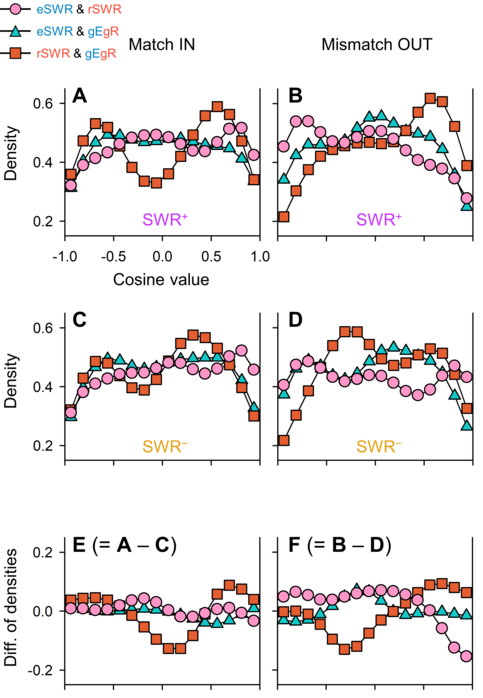
\includegraphics[width=0.5\textwidth]{./src/figures/.png/Figure_ID_07.png}
        	\caption{\DIFdelbeginFL \textbf{\DIFdelFL{Directions of Neural Trajectories during SWRs Based on Encoding and Retrieval States
}}
%DIFAUXCMD
\DIFdelendFL \DIFaddbeginFL \textbf{
\DIFaddFL{Neural Trajectories Direction during SWRs Based on Encoding and Retrieval States
}}
\DIFaddendFL \smallskip
\\
\textbf{\textit{A--B}} \DIFdelbeginFL \DIFdelFL{Kernel }\DIFdelendFL \DIFaddbeginFL \DIFaddFL{Shows the kernel }\DIFaddendFL density estimation distributions of \DIFdelbeginFL \DIFdelFL{$\protect\overrightarrow{{\mathrm{eSWR^+}}} \cdot \protect\overrightarrow{{\mathrm{rSWR^+}}}$ }\DIFdelendFL \DIFaddbeginFL \DIFaddFL{$\protect\overrightarrow{{\mathrm{eSWR^+}}}$ $\cdot$ $\protect\overrightarrow{{\mathrm{rSWR^+}}}$ }\DIFaddendFL (\DIFdelbeginFL \textit{\DIFdelFL{pink circles}}%DIFAUXCMD
\DIFdelendFL \DIFaddbeginFL \DIFaddFL{depicted as pink circles}\DIFaddendFL ), \DIFdelbeginFL \DIFdelFL{$\protect\overrightarrow{{\mathrm{eSWR^+}}} \cdot \protect\overrightarrow{{\mathrm{g_{E}g_{R}}}}$ }\DIFdelendFL \DIFaddbeginFL \DIFaddFL{$\protect\overrightarrow{{\mathrm{eSWR^+}}}$ $\cdot$ $\protect\overrightarrow{{\mathrm{g_{E}g_{R}}}}$ }\DIFaddendFL (\DIFdelbeginFL \textit{\DIFdelFL{blue triangles}}%DIFAUXCMD
\DIFdelendFL \DIFaddbeginFL \DIFaddFL{blue triangles}\DIFaddendFL ), and \DIFdelbeginFL \DIFdelFL{$\protect\overrightarrow{{\mathrm{rSWR^+}}} \cdot \protect\overrightarrow{{\mathrm{g_{E}g_{R}}}}$ }\DIFdelendFL \DIFaddbeginFL \DIFaddFL{$\protect\overrightarrow{{\mathrm{rSWR^+}}}$ $\cdot$ $\protect\overrightarrow{{\mathrm{g_{E}g_{R}}}}$ }\DIFaddendFL (\DIFdelbeginFL \textit{\DIFdelFL{red rectangles}}%DIFAUXCMD
\DIFdelendFL \DIFaddbeginFL \DIFaddFL{red rectangles}\DIFaddendFL ) in \DIFaddbeginFL \DIFaddFL{the }\DIFaddendFL Match In (\textit{A}) and Mismatch OUT tasks (\textit{B}). \textbf{\textit{C--D}} \DIFdelbeginFL \DIFdelFL{Present }\DIFdelendFL \DIFaddbeginFL \DIFaddFL{Illustrates }\DIFaddendFL the corresponding distributions of $\mathrm{SWR^-}$ instead of those of $\mathrm{SWR^+}$ in \textit{A} and \textit{B}. \textbf{\textit{E--F}} \DIFdelbeginFL \DIFdelFL{Depict }\DIFdelendFL \DIFaddbeginFL \DIFaddFL{Renders }\DIFaddendFL the differences in the distributions of $\mathrm{SWR^+}$ and $\mathrm{SWR^-}$, \DIFdelbeginFL \DIFdelFL{illuminating }\DIFdelendFL \DIFaddbeginFL \DIFaddFL{detailing }\DIFaddendFL the SWR components (\textit{E} = \textit{C} \DIFdelbeginFL \DIFdelFL{$-$ }\DIFdelendFL \DIFaddbeginFL \DIFaddFL{- }\DIFaddendFL \textit{A} \DIFdelbeginFL \DIFdelFL{\& }\DIFdelendFL \DIFaddbeginFL & \DIFaddendFL \textit{F} = \textit{D} \DIFdelbeginFL \DIFdelFL{$-$ }\DIFdelendFL \DIFaddbeginFL \DIFaddFL{- }\DIFaddendFL \textit{B}). \DIFdelbeginFL \DIFdelFL{Note the }\DIFdelendFL \DIFaddbeginFL \DIFaddFL{The }\DIFaddendFL biphasic distributions of \DIFdelbeginFL \DIFdelFL{$\protect\overrightarrow{{\mathrm{rSWR^-}}} \cdot \protect\overrightarrow{{\mathrm{g_{E}g_{R}}}}$, suggesting }\DIFdelendFL \DIFaddbeginFL \DIFaddFL{$\protect\overrightarrow{{\mathrm{rSWR^-}}}$ $\cdot$ $\protect\overrightarrow{{\mathrm{g_{E}g_{R}}}}$ indicates }\DIFaddendFL fluctuations between the encoding and retrieval states during the Sternberg task. \DIFdelbeginFL \DIFdelFL{Moreover}\DIFdelendFL \DIFaddbeginFL \DIFaddFL{Also}\DIFaddendFL , \DIFdelbeginFL \DIFdelFL{inverse }\DIFdelendFL \DIFaddbeginFL \DIFaddFL{contradicting }\DIFaddendFL directionality between $\protect\overrightarrow{{\mathrm{eSWR^+}}}$ and $\protect\overrightarrow{{\mathrm{rSWR^+}}}$ was observed (\DIFdelbeginFL \textit{\DIFdelFL{pink circles}}%DIFAUXCMD
\DIFdelendFL \DIFaddbeginFL \DIFaddFL{pink circles}\DIFaddendFL ) not in the Match IN task \DIFaddbeginFL \DIFaddFL{(}\DIFaddendFL \textbf{\textit{E}})\DIFdelbeginFL \DIFdelFL{) }\DIFdelendFL \DIFaddbeginFL \DIFaddFL{, }\DIFaddendFL but in Mismatch OUT task \DIFaddbeginFL \DIFaddFL{(}\DIFaddendFL \textbf{\textit{F}})\DIFaddbeginFL \DIFaddFL{. Lastly}\DIFaddendFL , \DIFdelbeginFL \DIFdelFL{Finally, shifts }\DIFdelendFL \DIFaddbeginFL \DIFaddFL{transition }\DIFaddendFL from the retrieval to encoding states are \DIFdelbeginFL \DIFdelFL{acknowledged }\DIFdelendFL \DIFaddbeginFL \DIFaddFL{apparent }\DIFaddendFL in the SWR components in both Match IN and Mismatch OUT tasks (\DIFdelbeginFL \textit{\DIFdelFL{red rectangles}} %DIFAUXCMD
\DIFdelendFL \DIFaddbeginFL \DIFaddFL{red rectangles }\DIFaddendFL in \textit{E--F}).
}
% width=0.5\textwidth
        	\label{fig:07}
        \end{figure*}

%%%%%%%%%%%%%%%%%%%%%%%%%%%%%%%%%%%%%%%%%%%%%%%%%%%%%%%%%%%%%%%%%%%%%%%%%%%%%%%%
%% END
%%%%%%%%%%%%%%%%%%%%%%%%%%%%%%%%%%%%%%%%%%%%%%%%%%%%%%%%%%%%%%%%%%%%%%%%%%%%%%%%

\end{document}
